\hyphenation{
Mit-ar-bei-ter-da-tei
Fund-da-tei
Be-fund-da-tei
Pro-jekt-da-tei
}
\paragraph{Übersicht}
Datenbanksysteme (DBS) werden zur Strukturierung, Pflege und Verwaltung von Daten verwendet. Sie bestehen aus zwei Komponenten - einerseits aus der Datenbank, welche den logisch zusammengehörigen Datenbestand umfasst, sowie aus dem  Datenbankmanagementsystem (DBMS), der Datenbanksoftware, welche u.a. die Zugriffsrechte regelt und Vorkehrungen zur Datensicherheit gewährleistet. Es gibt verschiedene Datenbankmodelle, von denen relationale Datenbanksysteme am häufigsten verwendet und im Rahmen der IT Empfehlungen betrachtet werden. Dabei werden die Daten in Tabellen (Relationen) strukturiert, wobei Verweise von einer Tabelle auf eine andere möglich sind. Näheres zu Tabellen ist in dem Kapitel Tabellen ab Seite \pageref{tabellen} zu finden.

\subparagraph{Langzeitformate}
Für relationale Datenbanken wird eine Archivierung in Form eines Exports der Datenbankinhalte, der Strukturinformationen und weiterer Funktionalitäten in textbasierte Formate empfohlen, welche unabhängig vom verwendeten Datenbankmanagementsystem sind. Neben den Daten in den Tabellen müssen die Datenbankstrukturdefinitionen wie Attributdatentypen, Relationen zwischen den Tabellen und Formeln zwingend mit archiviert werden. Unabhängig vom gewählten Archivformat ist es nötig, die grafische Benutzeroberfläche zu dokumentieren, zum Beispiel in Form von Bildschirmfotos oder eines eventuell vorhandenen Benutzerhandbuches. Eine darüberhinaus gehende Erhaltung der Funktionalität ist zumeist nur mit Hilfe der technisch sehr aufwendigen Emulation möglich, bei der das ursprüngliche Datenbanksystem durch ein anderes System mit ähnlicher Funktionsweise ersetzt wird. Unabhängig von den vorgestellten Archivformaten ist der Umgang mit sogenannten Binary Large Objects (BLOBs). Dabei handelt es sich um intern gespeicherte Mediendateien, meistens Fotos, Zeichnungen, z. B. von Funden, oder PDF-Dokumente. Diese Medien müssen in jedem Fall exportiert, auf die dann externen Dateien muss referenziert und je nach Dateityp in für die Archivierung geeigneten Formaten gespeichert werden (siehe entsprechendes Dateiformatkapitel). Grundsätzlich wird von der Verwendung von BLOBs abgeraten und eine externe Speicherung von Medieninhalten empfohlen.

Ein geeignetes Archivformat ist SQL (Structured Query Language), welches seit 1986 bei der ANSI standardisiert ist und seit 1987 ebenfalls als ISO/IEC 9075 zertifiziert ist. Seitdem wurde der SQL-Standard in sieben Revisionen weiter ausgebaut, wobei SQL:2011 die neueste Version ist. Jedoch wird dieser Standard in den verschiedenen Datenbanksystemen wie MySQL, PostgreSQL oder OracleDB unterschiedlich umgesetzt und erweitert. Daher gibt es je nach Datenbanksystem mehrere spezifische Befehle, welche über die Spezifikation des Standards hinausgehen. In Folge dessen sind die verschiedenen DBMS nicht vollständig kompatibel, weswegen eine exportierte Datenbank im SQL-Format nur dann problemlos und ohne zusätzlichen Aufwand importiert werden kann, wenn das ursprüngliche DBMS verwendet wird. Daher kann SQL für die Archivierung nur dann empfohlen werden, wenn ein einheitlicher ANSI-/ISO-Standard, z. B. SQL:2008, verwendet wird, welcher von DBMS-spezifischen Befehlen bereinigt ist. Der verwendete Standard muss dokumentiert werden. Der Vorteil in der Speicherung in SQL liegt in der gleichzeitigen Erhaltung der kompletten Daten, der Tabellen und ihrer Relationen zueinander, der Attributspezifikationen sowie der kompletten Metadaten. Nach einem Export, erhält man eine singuläre textbasierte Datei, welche sich mit relativ geringem Aufwand wiederherstellen lässt. Die Speicherung einer Datenbank in einem SQL-Skript erfolgt unter Angabe der SQL-Befehle, welche zum Import der Datenbankinhalte benötigt und ggf. für jeden Datensatz wiederholt werden müssen. Die damit einhergehende Redundanz erhöht die Datenmenge. Datenbanken aus geisteswissenschaftlichen Forschungsprojekten erreichen jedoch nur selten eine Größe, bei welcher dieser Nachteil zum Tragen kommt.

XML eignet sich als Archivformat für Datenbanken aus Gründen der Systemunabhängigkeit, Standardisierung, Lesbarkeit und Erweiterbarkeit. Für die Speicherung der Datenbankinhalte kann XML uneingeschränkt empfohlen werden. Die Beschreibung der Datenbankstruktur sollte mithilfe einer entsprechenden XML-Schema-Definition (XSD) wie der Database Markup Language erfolgen. Alternativ kann die Datenbankstruktur im SQL-Format und als Entitäten-Relationen-Diagramm (ERD) gespeichert werden.

Das 2008 initial vom schweizerischen Bundesarchiv entwickelte und im Rahmen des e-ARK-Projekts weiterentwickelte Format SIARD (Software Independent Archiving of Relational Databases) in der Version 2.0 beruht im Wesentlichen auf den beiden ISO-Standards XML gemäß ISO/IEC 19503:2005 und SQL:2008. Es vereinigt damit die Vorteile einer Datenhaltung in XML mit einer Dokumentation der Datenbankstruktur in SQL. Es ist als eCH-Standard offen und wird unter einer freien Lizenz zur Verfügung gestellt.

Ein alternativer bewährter Ansatz zur Archivierung der Tabellen einer Datenbank ist der Export in das CSV-Format, welches besonders langlebig und weit verbreitet ist. Diese Methode ist technisch mit relativ geringem Aufwand verbunden, besitzt aber einen starken Fokus auf die Datenbankinhalte und geht daher mit einem vollständigen Verlust der Funktionalitäten und Datenbankstruktur einher. Infolgedessen ist es zwingend erforderlich, bei der Speicherung im CSV-Format zusätzlich die Datenbankstruktur in Form von strukturierten Diagrammen, wie dem Entitäten-Relationen-Diagramm (ERD) festzuhalten. Selbst dann ist die Datenbankstruktur nur teilweise und sehr aufwendig rekonstruierbar, weswegen das CSV-Format nur bei einer hybriden Lösung mit der Archivierung der Datenbankstruktur in einem geeigneten Format (z. B. SIARD, SQL, XML/DML) bei gleichzeitiger Speicherung der Daten im CSV-Format, empfohlen werden kann. Als Zeichenkodierung sollte UTF-8 verwendet werden, wobei RFC-4180-konform als Trennzeichen ein Komma (\emph{,}) und als Textbegrenzungszeichen das Anführungszeichen (\emph{''}) verwendet werden sollte. Mehr dazu ist in dem Kapitel Tabellen ab Seite \pageref{tabellen} zu finden.

Bei der JavaScript Object Notation (JSON) handelt es sich um ein einfaches textbasiertes Datenformat, welches für einen schnellen Datentransfer im Internet entwickelt wurde und als RFC 7159 und ECMA-404 standardisiert ist. Es besitzt bei der Speicherung von Daten vergleichbare Vorteile wie XML, ist dabei aber wesentlich kompakter. Zur Zeit gibt es allerdings keinen Standard zur Beschreibung von Datenbankstrukturen in JSON, weswegen auch hier auf eine hybride Archivierungslösung mit der Speicherung der Datenbankinhalte in JSON und gleichzeitiger Speicherung der Datenbankstruktur in einem anderen Format (z. B. SIARD, SQL, XML/DML) zurückgegriffen werden muss.

Die proprietären Dateiformate von Desktop-DBMS, wie Microsoft Access, dBASE oder FileMaker eignen sich nicht für die Archivierung, da die Formatspezifikationen nicht offen vorliegen und verschiedene Versionen oft nicht untereinander kompatibel sind. Ebenso verhält es sich mit den binären Exportformaten serverbasierter, relationaler DBMS, wie Oracles DMP-Format oder das komprimierte BAK-Format von PostgreSQL. Auch diese folgen keinem allgemeingültigen Standard, liegen nur als Binärdatei vor und sind teilweise proprietär. Eine spätere Nachnutzung ist eng an das jeweilige für alle Nutzer kostenpflichtige Produkt sowie spezielle Tools gebunden.

ODB ist ein Container-Dateiformat des Programms, welche in LibreOffice und OpenOffice enthalten ist. ODB ist ein Teil vom OpenDocument Format (ODF) und wurde von einem technischen Komitee unter der Leitung der Organization for the Advancement of Structured Information Standards (OASIS) entwickelt und unter ISO/IEC 26300 standardisiert. Der ZIP-Container enthält verschiedene Dateien, die zum Betrieb der Datenbank erforderlich sind, wie persönliche Konfigurationsdateien, eine binäre Datei des Datenbankmanagementsystems HSQLDB mit den  Datenbankinhalten sowie der Datenbankstruktur und die XML-basierten Formulare und Reports. Aufgrund der binären Datenstruktur kann ODB nicht für die Langzeitarchivierung empfohlen werden.

Keines der genannten und empfohlenen Formate unterstützt und enthält alle notwendigen Informationen und signifikanten Eigenschaften, die für die Archivierung und Nachnutzung einer Datenbank relevant sind. Und einige Informationen, etwa ein Handbuch zur Benutzung, müssen ohnehin gesondert gespeichert werden. Daher ist eine hybride Archivierungsstrategie erforderlich, welche verschiedene Dateien mit unterschiedlichen Dateiformaten umfasst. In der folgenden Tabelle werden die Kategorien von Informationen, welche von den für die Archivierung geeigneten Datenbankformate prinzipiell gespeichert werden können, durch Abkürzungen kenntlich gemacht: I = Datenbankinhalt, S = Datenbankstruktur, F = Funktionalitäten, B = Benutzung. Eine zusätzliche Übersicht ist in dem Abschnitt Vertiefung zu finden.

\begin{center}
	\begin{longtable}{l L{0.2\textwidth} p{0.6\textwidth}}
			\toprule 
		\multicolumn{2}{l}{Format} & Begründung \\
		\midrule \endfirsthead
		\multicolumn{3}{l}{\footnotesize Fortsetzung der vorhergehenden Seite}\\
		\toprule
		\multicolumn{2}{l}{Format} & Begründung \\ \midrule \endhead
		\bottomrule \multicolumn{3}{r}{{\footnotesize Fortsetzung auf der nächsten Seite}} \\
		\endfoot
		\bottomrule 
		\endlastfoot
		
		\multirow{3}{*}{\color{ForestGreen} \LARGE \checkmark} & SIARD, SIARD2 & SIARD ist offen, frei verfügbar und setzt auf die Standards SQL und XML. Der wesentliche Vorteil von SIARD liegt darin, dass sowohl die Datenbankstruktur als auch die Datenbankinhalte gemeinsam beschrieben und archiviert werden. Für die Archivierung sollte Version 2.0 verwendet werden. Speichert: I, S, F.\\
			& SQL & Geeignet für die Langzeitarchivierung bei Verwendung eines offiziellen ISO/IEC 9075 Standards, z.B. SQL:2008. Daten, Datenbankstruktur und ein Großteil der Funktionalität bleiben erhalten. Der verwendete Standard muss dokumentiert sein. Speichert: I, S, F.\\
		  & XML & XML bietet sich insbesondere zur Speicherung der Daten einer Datenbank an. Die Datenbankstruktur sollte mit Hilfe eines XSD-Schemas, wie DBML, beschrieben werden. Alternativ ist dies auch mithilfe einer SQL-Datei oder SIARD möglich. Speichert I und teilweise S.\\ \cmidrule(r){1-3}
		\multirow{2}{*}{$\color{BurntOrange} \thicksim$} & CSV & Das CSV Format ist ein langlebiges, textbasiertes und weit verbreitetes Format. Bei dem Export von Datenbankinhalten in das CSV-Format gehen allerdings Informationen zur Datenbankstruktur und zu Funktionalitäten verloren, weshalb es nur bei einer gleichzeitigen Speicherung der Datenbankstruktur in einem anderen Format (z. B. SIARD, SQL, XML/DBML) zu empfehlen ist. Speichert: I.\\ 
			& JSON & JSON bietet sich als Format zur strukturierten Speicherung von Datenbankinhalten an. Da es keine Standards zur Beschreibung der Datenbankstruktur im JSON Format gibt, muss diese gesondert in einem geeigneten Format (z. B. SIARD, SQL, XML/DBML) gespeichert werden. JSON bietet sich insbesondere für die Archivierung von Daten aus NoSQL Datenbanken an. Speichert: I.\\ \cmidrule(r){1-3}
		\multirow{5}{*}{\LARGE \boldmath$\color{BrickRed} \times$}& MDB, ACCDB & Binäre, proprietäre Formate von Microsoft Access, die nicht zur Archivierung geeignet sind.\\
		& FP5, FP7, FMP12 & Binäre, proprietäre Formate von FileMaker, die nicht zur Archivierung geeignet sind.\\
		& ODB & Containerformat von OpenOffice, welches verschiedene XML-basierte Dateien, wie z.B. Formulare und Abfragen, und die binären Dateien mit den Inhalten und der Struktur der Datenbank enthält. ODB ist nicht zur Archivierung geeignet. Speichert: teilweise B.\\
		& DBF & Binäres, proprietäres Format von dBASE, das nicht zur Archivierung geeignet ist.\\
		& BAK, DB, DMP & Die verschiedenen, binären Exportformate von relationalen Datenbanksystemen sind für die Archivierung nicht geeignet.\\
		\bottomrule    
	\end{longtable}
\end{center}


\subparagraph{Dokumentation}
Die Empfehlungen zur Dokumentation von Datenbanken orientieren sich an verschiedenen Standards, darunter SIARD Metadata Schema, Archival Data Description Mark-up Language (ADDML) und Database Markup Language (DBML). Allen Schemata gemein ist eine differenzierte Beschreibung der verschiedenen Ebenen eines Datenbanksystems. Dazu gehören Metadaten zur allgemeinen Beschreibung der Datenbank als auch spezifische Metadaten zur Beschreibung der hierarchisch aufgebauten Ebenen einer Datenbank: den in SQL Datenbanken vorkommenden Schemen, die mehrere Tabellen beinhalten, welche wiederum mit Hilfe von mehreren Attributen definiert werden können. 

Weitergehende Dokumente, die zum Verständnis einer Datenbank, ihrer spezifischen Nutzung oder zur Eigenart der Inhalte notwendig sind, wie beispielsweise Benutzerhandbuch, Bildschirmfotos, ERD-Diagramme, Beschreibungen semantischer Konventionen (wie Wertelisten), Anforderungsanalysen oder Rechte- und Rollendokumentation sollten auf alle Fälle mit archiviert werden.

Ergänzend zu den Metadaten, wie sie in dem Abschnitt Metadaten in der Anwendung ab Seite \pageref{Metadaten-anwendung} gelistet sind, sollten folgende minimale Metadaten zur nachhaltigen Beschreibung von Datenbanken aufgenommen werden.

\begin{center}
	\begin{longtable}{L{0.3\textwidth} p{0.6\textwidth}}
			\toprule 
		Metadatum & Beschreibung \\
		\midrule \endfirsthead
		\multicolumn{2}{l}{\footnotesize Fortsetzung der vorhergehenden Seite}\\
		\toprule
		Metadatum & Beschreibung \\ \midrule \endhead
		\bottomrule \multicolumn{2}{r}{{\footnotesize Fortsetzung auf der nächsten Seite}} \\
		\endfoot
		\bottomrule 
		\endlastfoot
		
		Datenbankname & Ansprache/Name der Datenbank\\
		Beschreibung der Datenbank & Zusammenfassung über Zweck, Bedeutung und Inhalt der Datenbank\\
		Sprache & Liste der Sprachen, in welchen die Daten eingegeben wurden sowie Sprachkennungen nach ISO 639 angeben.\\
		Identifikator & Falls die Datenbank online öffentlich zugänglich ist, sollte ein persistenter Identifikator (z.B. DOI, URI) oder eine eindeutige Adresse (z.B. URL) angegeben werden.\\
		Rechteinhaber & Personen, Institutionen oder Unternehmen, die Rechte an der Datenbankstruktur und/oder den Datenbankinhalten besitzen.\\
		DBMS & Name des Datenbankmanagementsystems mit Versionsnummer mit der die Datenbank betrieben wurde.\\
		Schemata Liste & Liste der Schemata innerhalb der Datenbank sofern vorhanden.\\
		Benutzer & Liste der Benutzer und ihrer Rolle innerhalb der Datenbank.\\
		Rolle & Liste der verschiedenen Rollen und Gruppen mit ihren definierten Zugriffsrechten.\\
		Standard & Name und Version verwendeter Standards, etwa zur Definition des Datentyps eines Attributs, zur Dokumentation von Abfragen oder zu dem Datenbankformat, z.B. SQL:2008 oder SIARD 2.0.\\
		Abgeleitete Dateien & Aus den Datenbankinhalten erzeugte Grafiken, Abbildungen, Diagramme müssen zusätzlich separat archiviert und gelistet werden.\\
		Weitere Dateien & Liste weiterer Dokumente, die für das Verständnis und die Dokumentation einer Datenbank notwendig sind, wie beispielsweise ein ERD oder ein Benutzerhandbuch.\\
		\midrule
		Schema Metadatum & Beschreibung\\
		Schema Name & Name des Schemas.\\
		Schema Beschreibung & Bedeutung und Inhalt des Schemas.\\
		Tabellenliste & Liste der Tabellen im Schema.\\
		Funktion & Name und Art der Funktion (Gespeicherte Funktionen, Sichten).\\
		Funktion Beschreibung & Beschreibung der Funktion hinsichtlich Sinn und Zweck.\\
		Funktion Befehl & Befehle der Funktion nach einem einheitlich festgelegten Standard (Syntax Standard).\\
		\midrule
		Tabelle Metadatum & Beschreibung\\
		Tabelle Name & Name der Tabelle.\\
		Tabelle Beschreibung & Bedeutung und Inhalt der Tabelle.\\
		Anzahl Datensätze & Anzahl der Datensätze in der Tabelle.\\
		Attributliste & Liste der Attribute in der Tabelle.\\
		\midrule
		Attribut Metadatum & Beschreibung\\
		Attribut Name & Name des Attributs.\\
		Attribut Beschreibung & Bedeutung und Inhalt des Attributs. Wird das Attribut mit Hilfe von Einheiten, z. B. metrische Maßeinheiten, ausgedrückt, ist die Angabe der Einheit erforderlich.\\
		Attribut Typ & Datentyp des Attributs nach einem einheitlich festgelegtem Standard (Syntax Standard) z. B. "`Integer"' nach SQL:2008.\\
		Kontrolliertes Vokabular & Sofern für das Attribut eine Werteliste vorliegt oder ein Thesaurus verwendet wurde, ist dieses zu dokumentieren.\\
		Attribut Schlüssel & Sofern es sich um ein Schlüsselattribut handelt, Benennung der Schlüsselart z. B. Primär- oder Fremdschlüssel. \\
		Fremdschlüssel Referenz & Im Falle eines Fremdschlüssels Angabe des referenzierten Attributs mit Angabe der Tabelle und des Schemas. \\

	  \bottomrule
	\end{longtable}
\end{center}


%###########################################################

\paragraph{Vertiefung}
Ein Datenbanksystem (DBS) ist ein System zur elektronischen Verwaltung großer Datenmengen, um diese effizient, widerspruchsfrei und dauerhaft zu speichern und in den benötigten Teilmengen in unterschiedlichen Darstellungsformen für Benutzer und Anwendungsprogramme bereitzustellen. Gegenüber einer Speicherung in strukturierten Einzeldateien, wie Tabellen, werden unter anderem folgende Probleme effizienter gelöst:

\begin{itemize}
	\item \textbf{Redundanzen:} Bei einer Speicherung in Einzeldateien werden viele Daten mehrfach gespeichert. Änderungen werden dadurch sehr aufwendig, da sie an verschiedenen Stellen durchgeführt werden müssen.
	\item \textbf{Inkonsistenzen:} Sowohl bei der gleichzeitigen Änderung von Daten durch mehrere Benutzer als auch bei Änderungen von redundanten Daten kann es leicht zu Widersprüchen und Inkonsistenzen in den Daten kommen, was mit der Verwendung von DBS vermieden wird.
	\item \textbf{Integritätsbedingungen:} Sofern einzelne oder globale Informationen direkt von anderen Informationen abhängen, lassen sich entsprechende Bedingungen in der Datenbank abbilden, die bei der Eingabe neuer Informationen eine Kontrollfunktion übernehmen und dadurch bestimmte Fehler in den Daten verhindern können.
	\item \textbf{Datenschutzprobleme:} Einzeldateien besitzen kein dezidiertes User"=Management, weswegen ein Zugriff auf den gesamten Datenbestand vorliegt, wohingegen DBS differenzierte Zugriffsregelungen ermöglichen.
	\item \textbf{Darstellungsvarianten:} Mit einem DBS lassen sich verschiedene Ausschnitte, sog. Sichten (engl. views), aus der Gesamtmenge aller gespeicherten Informationen erstellen und so einmal eingetragene Informationen für unterschiedliche Zwecke und Nutzer variabel anzeigen (z.B. in einem Eingabeformular, als tabellarische Übersicht oder vorformatiert für eine Publikation).
\end{itemize}

Ein DBS besteht aus der Verwaltungssoftware, genannt Datenbankmanagementsystem (DBMS), und der Menge der zu verwaltenden Informationen, der eigentlichen Datenbank (DB). Die Datenbank enthält zusätzlich zu den eigentlichen Inhalten noch die Beschreibung der Datenstruktur, die in einem Datenkatalog und in einem Datenbankschema mittels Metadaten festgehalten wird.

\tikzset{
		%Define standard arrow tip
    >=stealth',
		% Define arrow style
    pfeil/.style={
           >=stealth',
           draw=ianusBlau, very thick,
           shorten <=0.8em,
           shorten >=0.8em
					},
    %Define style for boxes
		abgerundetAussen/.style={
           rectangle,
           rounded corners,
           draw=ianusBlau, very thick,
					 inner xsep=0.5em,
					 minimum height=3em,
					 minimum width=10em,
           text centered	
					},
		abgerundetAussenSchmaler/.style={
           rectangle,
           rounded corners,
           draw=ianusBlau, very thick,
					 inner xsep=0.5em,
					 minimum height=4em,
					 minimum width=5em,
					 text width = 6.5em,
           text centered	
					},
    abgerundet/.style={
           rectangle,
           rounded corners,
           draw=ianusGrau, very thick,
					 fill=ianusGrau,
           minimum height=2em,
           text centered
					},
		abgerundetSchmaler/.style={
           rectangle,
           rounded corners,
           draw=ianusGrau, very thick,
					 fill=ianusGrau,
					 text width = 3.5em,
           text centered
					},
		% Define line style
    linie/.style={
           draw=ianusBlau, very thick,
					},
    %Define style for boxes
		eckigeBox/.style={
           rectangle,
           draw=ianusBlau, very thick,
					 fill=white,
					 %fill opacity=.9,
					 text opacity=1,
					 inner xsep=0.5em,
					 minimum height=0.7cm,
					 minimum width=2.5cm,
           text centered
					},
		raute/.style={
					 diamond,
					 aspect=2,
					 minimum width=2cm,
					 minimum height=0.8cm,
					 draw=ianusBlau, very thick,
		},
		ellipseDick/.style={
					 ellipse,
					 aspect=2,
					 minimum width=3cm,
					 minimum height=0.7cm,
					 draw=ianusBlau, very thick,
		}
}
\begin{figure}[h!tb]
	\begin{center}
	\resizebox{1\textwidth}{!}{%
	\begin{tikzpicture}[remember picture, node distance=1cm, auto]
		\node[abgerundetAussen] (dbs) {
			\begin{tikzpicture}
				\node[] (dbsLabel) {Datenbanksystem (DBS)};
				\node[abgerundet, below =0.2cm  of dbsLabel, align=center] (DBMS) {Datenbankmanagementsystem \\ (DBMS)};
				\node[abgerundet, below =2cm  of DBMS] (DB) {Datenbank (DB)};
			\end{tikzpicture}
		};
		\node[abgerundetAussenSchmaler, above left = 1.5cm and -2.6cm of dbs] (dbDoku) {Programm zur Grabungsdokumentation};
		\node[abgerundetAussenSchmaler, above right = 1.5cm and -2.7cm of dbs] (dbVerwaltung) {Programm zur Projektverwaltung};	
	
		\node[abgerundetAussenSchmaler, left = 0.5cm of dbDoku] (dateiVerwaltung) {Programm zur Projektverwaltung};
		\node[abgerundetAussenSchmaler, left = 0.5cm of dateiVerwaltung] (dateiDoku) {Programm zur Grabungsdokumentation};
		
		\node[abgerundetSchmaler, below left =1.5cm and -1.2cm of dateiDoku] (foto) {Foto-datei};
		\node[abgerundetSchmaler, below =2.5cm of dateiDoku] (befund) {Befund-datei};
		\node[abgerundetSchmaler, below right =3.5cm and -0.9cm of dateiDoku] (fund) {Fund-datei};
		
		\node[abgerundetSchmaler, below left =1.5cm and -1.0cm of dateiVerwaltung] (projektDat) {Projekt-datei};
		\node[abgerundetSchmaler, below right =2.5cm and -2.0cm of dateiVerwaltung] (mitarbeiterDat) {Mitar-beiter-datei};
		
		\path[pfeil, <->] (dateiDoku) edge [bend left=0] (foto);
		\path[pfeil, <->] (dateiDoku) edge [bend left=0] (befund);
		\path[pfeil, <->] (dateiDoku) edge [bend left=0] (fund);
		\path[pfeil, <->] (dateiDoku) edge [bend right=0] (projektDat);
	
		\path[pfeil, <->] (dateiVerwaltung) edge [bend right=0] (projektDat);
		\path[pfeil, <->] (dateiVerwaltung) edge [bend right=0] (mitarbeiterDat);
		
		\path[pfeil, <->] (dbDoku) edge [bend right=0] (dbs);
		\path[pfeil, <->] (dbVerwaltung) edge [bend right=0] (dbs);
		
		\path[pfeil, <->] (DBMS) edge [bend right=0] (DB);
		
	\end{tikzpicture}
	}%
	\end{center}
	\caption{Vergleich von Datenhaltung in Einzeldateien (links) gegenüber Datenhaltung mit Hilfe eines Datenbanksystems (rechts).}
	\label{abb:datenbanken-vergleich}
\end{figure}

Bei einem DBMS handelt es sich um ein Programm (kommerzielle Produkte sind u. a. FileMakerPro, Access und Oracle, OpenSource sind u. a. MySQL und PostgreSQL), das als Steuerungsprogramm intern die strukturierte Speicherung der Daten organisiert und alle lesenden und schreibenden Zugriffe auf die Datenbank ausführt. Der Benutzer greift also nicht direkt auf die Datenbank zu, sondern auf das DBMS als Kontrollinstanz. Die Aufgaben eines DBMS umfassen u. a. folgende Bereiche:

\begin{itemize}
	\item Eingabe, Änderung und Löschen von Daten
	\item Erstellen von Datenbanken inklusive Umsetzung des Datenmodells
	\item Suchen in den Datenbankinhalten mittels Abfragen
	\item generelle Verwaltung von Benutzern, Zugriffen und Zugriffsrechten
\end{itemize}

Der Begriff Datenbank (DB) bezieht sich auf die eigentlichen Sachdaten, die entweder von Benutzern manuell eingegeben oder automatisch generiert werden. Die Datenbankinhalte können in unterschiedlichen Formaten vorliegen und als Texte, Zahlen, Links oder Medien (Fotos, Zeichnungen, Filme etc.) in die Datenbank einfließen. Dieser Datenbestand wird von einem DBMS verwaltet, auf Speichermedien abgelegt und je nach Vorgabe kontrolliert (damit z. B. ein Funddatum immer auch einem Fund zugeordnet ist).


\subparagraph{Datenbankmodelle}
Zur formalen Beschreibung aller in der Datenbank enthaltenen Daten, ihrer Speicherung und ihrer Beziehungen untereinander verwendet man auf der konzeptionellen Ebene ein Datenmodell. Es ist die konzeptuelle Grundlage für ein Datenbanksystem und legt fest, auf welche Art und Weise der jeweils interessierende Ausschnitt aus der realen Welt in einer Datenbank abgebildet wird.
 
Es gibt verschiedene Datenmodelle, von denen das relationale das am weitesten verbreitete ist.

{\bfseries Relationales Datenmodell:} Bei Relationalen Datenbanken (Abbildung \ref{abb:datenbanken-relational}) werden die Daten sowie deren Beziehungen untereinander in Form von Tabellen (Relationen) beschrieben. Die einzelnen Einträge in unterschiedlichen Tabellen können mittels Verweise miteinander in Beziehung gesetzt werden.

\tikzstyle{backgroundRec}=[rectangle,
	fill=ianusGrau,
	inner sep=0cm]

\begin{figure}[h!tb]
	\begin{center}
	\begin{tikzpicture}[node distance=1cm, auto]
		\node[eckigeBox](fundst1){\tiny Fundstelle};
		\node[raute, below =0.8cm of fundst1](bezFund1){\tiny ist Fundort von};
		\node[eckigeBox, below =0.8cm of bezFund1](muenze1){\tiny Münze};
		\node[raute, below =0.8cm of muenze1](bezdok1){\tiny dokumentiert};
		\node[eckigeBox, below =0.8cm of bezdok1](foto1){\tiny Foto};
		\node[below =0.9cm of foto1](label1){ER-Modell Darstellung};
		
		\path[linie] (fundst1) edge node [near start] {\scriptsize 1} (bezFund1);
		\path[linie] (bezFund1) edge node [near end] {\scriptsize n} (muenze1);
		\path[linie] (muenze1) edge node [near start] {\scriptsize m} (bezdok1);
		\path[linie] (bezdok1) edge node [near end] {\scriptsize n} (foto1);
		
		\matrix[right =3.8cm of fundst1, row sep=0.05cm,column sep=0.05cm] (fundTab) {
				% Erste Zeile Fundstelle
        \node (1-1) [fill=ianusGrau]{\tiny ID}; &
        \node [fill=ianusGrau]{\tiny Name}; &
        \node [fill=ianusGrau]{\tiny Breite}; &
				\node (1-2) [fill=ianusGrau]{\tiny Länge}; &
        \\
        % Zweite Zeile Fundstelle
        \node []{\tiny 001}; &
        \node []{\tiny Korinth}; &
        \node []{\tiny 37.91}; &
				\node []{\tiny 22.87}; &
        \\
				% Dritte Zeile Fundstelle
        \node []{\tiny 002}; &
        \node []{\tiny Pergamon}; &
        \node []{\tiny 39.13}; &
				\node []{\tiny 27.18}; &
        \\
				% Vierte Zeile Fundstelle
        \node (fundst2) []{\tiny \dots}; &
        \node []{\tiny \dots}; &
        \node []{\tiny \dots}; &
				\node []{\tiny \dots}; &
        \\
		};
		\node[above left =0.0cm and -1.4cm of fundTab] {\tiny Fundstelle};
		
		\matrix[below right=0.6cm and -7.1cm of fundTab, row sep=0.05cm,column sep=0.05cm] (muenzeTab) {
				% Erste Zeile Münze
        \node (2-1) []{\tiny ID}; &
        \node []{\tiny Name}; &
        \node (fundID) []{\tiny Fundort-ID}; &
				\node (2-2) []{\tiny Metall}; &
        \\
        % Zweite Zeile Münze
        \node []{\tiny 0023}; &
        \node []{\tiny Commodus aus Korinth}; &
        \node []{\tiny 001}; &
				\node []{\tiny Bronze}; &
        \\
				% Dritte Zeile Münze
        \node []{\tiny 0024}; &
        \node []{\tiny Münze aus Korinth}; &
        \node []{\tiny 001}; &
				\node []{\tiny Bronze}; &
        \\
				% Vierte Zeile Münze
        \node (muenze2) []{\tiny \dots}; &
        \node []{\tiny \dots}; &
        \node []{\tiny \dots}; &
				\node []{\tiny \dots}; &
        \\
		};
		\node[above left =0.0cm and -1cm of muenzeTab] {\tiny Münze};
		
		\matrix[below left= 0.8cm and -2.7cm of muenzeTab, row sep=0.05cm,column sep=0.05cm] (dokuTab) {
				% Erste Zeile dokumentiert
        \node (3-1) []{\tiny Münze-ID}; &
				\node (3-2) []{\tiny Foto-ID}; &
        \\
        % Zweite Zeile dokumentiert
        \node []{\tiny 0023}; &
				\node []{\tiny 0049}; &
        \\
				% Dritte Zeile dokumentiert
        \node []{\tiny 0023}; &
				\node []{\tiny 0050}; &
        \\
				% Vierte Zeile dokumentiert
        \node []{\tiny 0024}; &
				\node []{\tiny 0051}; &
        \\
				% Fünfte Zeile dokumentiert
        \node []{\tiny \dots}; &
				\node (doku2)[]{\tiny \dots}; &
        \\
		};
		\node[above left =0.0cm and -1.7cm of dokuTab] {\tiny dokumentiert};
		
		\matrix[below right=0.8cm and -3cm of muenzeTab, row sep=0.05cm,column sep=0.05cm] (fotoTab) {
				% Erste Zeile Foto
        \node (4-1) []{\tiny ID}; &
				\node []{\tiny Name}; &
				\node (4-2) []{}; &
        \\
        % Zweite Zeile Foto
        \node []{\tiny 0049}; &
				\node []{\tiny Fundfoto - Avers}; &
				\node []{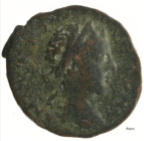
\includegraphics[width=.05\textwidth]{bilder/datenbanken_bsp1MA.jpg}}; &
        \\
				% Dritte Zeile Foto
        \node []{\tiny 0050}; &
				\node []{\tiny Fundfoto - Revers}; &
				\node []{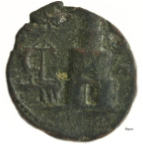
\includegraphics[width=.05\textwidth]{bilder/datenbanken_bsp1MR.jpg}}; &
        \\
				% Vierte Zeile Foto
        \node []{\tiny 0051}; &
				\node []{\tiny Fundfoto}; &
				\node []{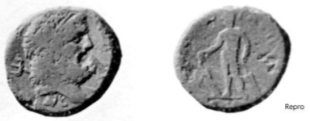
\includegraphics[width=.15\textwidth]{bilder/datenbanken_bsp2MAR.jpg}}; &
        \\
				% Fünfte Zeile Foto
        \node []{\tiny \dots}; &
				\node []{\tiny \dots}; &
				\node []{\tiny \dots}; &
        \\
		};
		\node[above left =0.0cm and -0.8cm of fotoTab] {\tiny Foto};
		
		\node[below =0.73cm of fotoTab](label2){Darstellung mit Beispielen};
		
		\begin{pgfonlayer}{background}
			\node [backgroundRec, fit=(1-1) (1-2)] {};
			\node [backgroundRec, fit=(2-1) (2-2)] {};
			\node [backgroundRec, fit=(3-1) (3-2)] {};
			\node [backgroundRec, fit=(4-1) (4-2)] {};
		\end{pgfonlayer}
		
		\draw[linie, dashed] (fundst2) -- (fundID);
		\draw[linie, dashed] (muenze2.south) -- (3-1.north);
		\draw[linie, dashed] (doku2.east) -- (4-1.west);
	\end{tikzpicture}
	\end{center}
	\caption{Beispiel einer relationalen Datenbank anhand von Münzdaten}
	\label{abb:datenbanken-relational}
\end{figure}


{\bfseries Hierarchisches Datenmodell:} Bei hierarchischen Datenbanken (Abbildung \ref{abb:datenbanken-hierarchisch}) werden die Informationen in Datensätze gruppiert und in einer baumartigen Datenstruktur gespeichert, die einer Mutter-Kind-Beziehung entspricht: Jede Mutter kann mehrere Kinder haben, ein Kind aber nur eine Mutter besitzen.

\begin{figure}[h!tb]
	\begin{center}
	\begin{tikzpicture}[node distance=1cm, auto]
		\node[eckigeBox](fundort){\tiny Fundort};
		\node[eckigeBox, below =0.8cm of fundort](muenze){\tiny Münze};
		\node[eckigeBox, below =0.8cm of muenze](foto){\tiny Foto};
		\node[below =5cm of fundort](label1){Allgemeine Darstellung};
		
		\draw[->, pfeil, shorten <=0em, shorten >=0em] (fundort) -- (muenze);
		\draw[->, pfeil, shorten <=0em, shorten >=0em] (muenze) -- (foto);

		\node[eckigeBox, right=3.8cm of fundort] (fundortBsp) {\tiny Korinth  Griechenland};
		\node[eckigeBox, below left=0.8cm and -0.6cm of fundortBsp](muenzeBsp1){\shortstack{\tiny Münze - Commodus\\ \tiny aus Korinth}};
		\node[eckigeBox, below left=0.8cm and -1.2cm of muenzeBsp1, minimum width=2cm](fotoBsp1a){\tiny Foto - Avers};
		\node[below=0.1cm of fotoBsp1a]{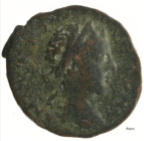
\includegraphics[width=.1\textwidth]{bilder/datenbanken_bsp1MA.jpg}};
		\node[eckigeBox, below right=0.8cm and -1.2cm of muenzeBsp1, minimum width=2cm](fotoBsp1b){\tiny Foto - Revers};
		\node[below=0.1cm of fotoBsp1b]{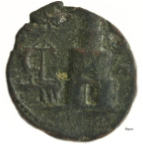
\includegraphics[width=.1\textwidth]{bilder/datenbanken_bsp1MR.jpg}};
		
		\node[eckigeBox, below right=0.8cm and -0.6cm of fundortBsp](muenzeBsp2){\tiny Münze aus Korinth};
		\node[eckigeBox, below=0.8cm of muenzeBsp2](fotoBsp2){\tiny Foto};
		\node[below=0.1cm of fotoBsp2]{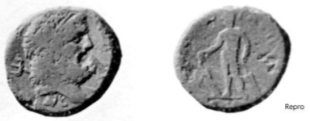
\includegraphics[width=.22\textwidth]{bilder/datenbanken_bsp2MAR.jpg}};
		\node[below =5cm of fundortBsp](label2){Darstellung mit Beispielen};
		
		\draw[->, pfeil, shorten <=0em, shorten >=0em] (fundortBsp) -- (muenzeBsp1);
		\draw[->, pfeil, shorten <=0em, shorten >=0em] (fundortBsp) -- (muenzeBsp2);
		\draw[->, pfeil, shorten <=0em, shorten >=0em] (muenzeBsp1) -- (fotoBsp1a);
		\draw[->, pfeil, shorten <=0em, shorten >=0em] (muenzeBsp1) -- (fotoBsp1b);
		\draw[->, pfeil, shorten <=0em, shorten >=0em] (muenzeBsp2) -- (fotoBsp2);
	\end{tikzpicture}
	\end{center}
	\caption{Beispiel einer hierarchischen Datenbank anhand von Münzdaten}
	\label{abb:datenbanken-hierarchisch}
\end{figure}

{\bfseries Netzwerk Datenmodell:} Netzwerkdatenbanken (Abbildung \ref{abb:datenbanken-netzwerk}) stellen eine Verallgemeinerung und Weiterentwicklung des hierarchischen Datenmodells dar, wobei die Daten in logischen Graphen strukturiert werden. Da die einzelnen Knoten im Graph beliebig miteinander über Beziehungen verknüpft werden könne, entfallen die Beschränkungen, die mit Mutter-Kind-Beziehungen einhergehen.

\begin{figure}[h!tb]
	\begin{center}
	\begin{tikzpicture}[node distance=1cm, auto]
		\node[eckigeBox](foto){\tiny Foto};
		\node[eckigeBox, below =0.3cm of foto](fotoA){\tiny Foto - Avers};
		\node[eckigeBox, below =0.3cm of fotoA](fotoR){\tiny Foto - Revers};
		\node[eckigeBox, below =1.0cm of fotoR](foto2){\tiny Foto};
		\node[eckigeBox, below right=2.0cm and 0.5cm of foto, inner sep=0.1pt](collection){\shortstack{\tiny American Numismatic\\ \tiny Society,\\ \tiny Newell Collection}};
		
		\node[eckigeBox, left=0.8cm of foto] (muenze1) {\shortstack{\tiny Münze \\ \tiny des Mark Aurel}};
		\node[eckigeBox, below=0.8cm of muenze1](muenze2){\shortstack{\tiny Münze - Commodus\\ \tiny aus Korinth}};
		\node[eckigeBox, below=1.1cm of muenze2](muenze3){\tiny Münze aus Korinth};
		\node[eckigeBox, below left=0.2cm and 0.1cm of muenze2](ort){\shortstack{\tiny Korinth \\ \tiny (Griechenland)}};
		\node[eckigeBox, below left=0.7cm and -1.0cm of muenze3](katalog){\shortstack{\tiny Katalog\\ \tiny Torsten Bendschus}};
		
		\begin{scope}[on background layer]
			\draw[->, pfeil, shorten <=0em, shorten >=0em] (collection) -- (foto.east);
			\draw[->, pfeil, shorten <=0em, shorten >=0em] (collection) -- (fotoA.east);
			\draw[->, pfeil, shorten <=0em, shorten >=0em] (collection) -- (fotoR.east);
			\draw[->, pfeil, shorten <=0em, shorten >=0em] (collection) -- (muenze1.east);
			\draw[->, pfeil, shorten <=0em, shorten >=0em] (collection) -- (muenze2.east);
			\draw[->, pfeil, shorten <=0em, shorten >=0em] (collection) -- (muenze3.east);
			
			\draw[->, pfeil, shorten <=0em, shorten >=0em] (muenze1) -- (foto.west);
			\draw[->, pfeil, shorten <=0em, shorten >=0em] (muenze2) -- (fotoA.west);
			\draw[->, pfeil, shorten <=0em, shorten >=0em] (muenze2) -- (fotoR.west);
			\draw[->, pfeil, shorten <=0em, shorten >=0em] (muenze3) -- (foto2.west);
			
			\draw[->, pfeil, shorten <=0em, shorten >=0em] (ort) -- (muenze2.west);
			\draw[->, pfeil, shorten <=0em, shorten >=0em] (ort) -- (muenze3.west);
			
			\draw[->, pfeil, shorten <=0em, shorten >=0em] (katalog) -- (muenze1);
			\draw[->, pfeil, shorten <=0em, shorten >=0em] (katalog) -- (muenze2);
			\draw[->, pfeil, shorten <=0em, shorten >=0em] (katalog) -- (muenze3);
		\end{scope}
	\end{tikzpicture}
	\end{center}
	\caption{Beispiel einer Netzwerkdatenbank anhand von Münzdaten}
	\label{abb:datenbanken-netzwerk}
\end{figure}

{\bfseries Objektorientiertes Datenmodell:} Analog zu den objektorientierten Programmiersprachen versuchen objektorientierte Datenbanken (Abbildung \ref{abb:datenbanken-objektorientiert}) Objekte aus der realen Welt mit ihren Eigenschaften und ihrem Verhalten nachzubilden. Die Definition der Objekte erfolgt über Klassen, welche Attribut- und Verhaltensdefinitionen enthalten und als Bauplan für daraus erzeugte Objekte fungieren.

\begin{figure}[h!tb]
	\begin{center}
	\resizebox{1\textwidth}{!}{%
	\begin{tikzpicture}[remember picture, node distance=1cm, auto]
		\matrix[row sep=0.0cm,column sep=0.05cm, column 1/.style={anchor=base west}] (fundort) {
        \node (fo-1) [fill=ianusGrau, font=\bfseries, text width=2.7cm]{\scriptsize Klasse Fundort};
        \\
        \node []{\tiny //Attribute}; \\
        \node [font=\bfseries]{\tiny ID}; \\
        \node [font=\bfseries]{\tiny Name}; \\
				\node [font=\bfseries]{\tiny Breite}; \\
				\node [font=\bfseries]{\tiny Länge}; \\
				\node []{}; \\
				\node []{\tiny //Beziehungen}; \\
				\node [text width=2.7cm] (fo-9) {\tiny istFundortVon <Münze>}; \\
		};
		\draw [ianusGrau] (fo-1.north west) -- (fo-1.north east) -- (fo-9.south east) -- (fo-9.south west) -- cycle ;
		
		\matrix[right=2.0cm of fundort, row sep=0.0cm,column sep=0.05cm, column 1/.style={anchor=base west}] (muenze) {
        \node (m-1) [fill=ianusGrau, font=\bfseries, text width=3.45cm]{\scriptsize Klasse Münze};
        \\
        \node []{\tiny //Attribute}; \\
        \node [font=\bfseries]{\tiny ID}; \\
        \node [font=\bfseries]{\tiny Name}; \\
				\node [font=\bfseries]{\tiny Metall}; \\
				\node []{}; \\
				\node []{\tiny //Beziehungen}; \\
				\node []{\tiny wurdeGefundenIn <Fundort>}; \\
				\node [text width=3.45cm] (m-9) {\tiny wurdeDokumentiertVon <Foto>}; \\
		};
		\draw [ianusGrau] (m-1.north west) -- (m-1.north east) -- (m-9.south east) -- (m-9.south west) -- cycle ;
		
		\matrix[right=2.5cm of muenze, row sep=0.0cm,column sep=0.05cm, column 1/.style={anchor=base west}] (foto) {
        \node (f-1) [fill=ianusGrau, font=\bfseries, text width=2.6cm]{\scriptsize Klasse Foto};
        \\
        \node []{\tiny //Attribute}; \\
        \node [font=\bfseries]{\tiny ID}; \\
        \node [font=\bfseries]{\tiny Name}; \\
				\node []{}; \\
				\node []{\tiny //Beziehungen}; \\
				\node [text width=2.6cm] (f-9) {\tiny dokumentiert <Münze>}; \\
		};
		\draw [ianusGrau] (f-1.north west) -- (f-1.north east) -- (f-9.south east) -- (f-9.south west) -- cycle ;
		
		\draw[*-*, draw=ianusBlau, fill=ianusBlau, shorten <=-0.4em, shorten >=-0.4em ] (fundort) to node[pos=0.35]{\tiny istFundortVon} node[pos=0.55, below]{\tiny wurdeGefundenIn} (muenze);
		\draw[*-*, draw=ianusBlau, fill=ianusBlau, shorten <=-0.4em, shorten >=-0.4em ] (muenze) to node[pos=0.5]{\tiny wurdeDokumentiertVon} node[near end, below]{\tiny dokumentiert} (foto);
		
		\node[below left=0cm and -8.2cm of fundort]{Darstellung im objektorientierten Datenbankschema};
	\end{tikzpicture}
	}%	
	
	\resizebox{1\textwidth}{!}{%
	\begin{tikzpicture}[remember picture, node distance=1cm, auto]
		\matrix[row sep=0.0cm,column sep=0.05cm, column 1/.style={anchor=base west}] (fundortBsp) {
        \node [font=\bfseries, text width=1.8cm] (fo-1Bsp) {\tiny ID: 001}; \\
        \node [font=\bfseries]{\tiny Name: Korinth}; \\
				\node [font=\bfseries]{\tiny Breite: 37.91}; \\
				\node [font=\bfseries]{\tiny Länge: 22.87}; \\
				\node []{}; \\
				\node [text width=1.8cm] (fo-9Bsp) {\tiny istFundortVon}; \\
		};
		\draw [ianusGrau] (fo-1Bsp.north west) -- (fo-1Bsp.north east) -- (fo-9Bsp.south east) -- (fo-9Bsp.south west) -- cycle ;
		
		\matrix[right=1.2cm of fundortBsp, row sep=0.0cm,column sep=0.05cm, column 1/.style={anchor=base west}] (muenzeBsp) {
        \node [font=\bfseries, text width=2.5cm] (m-1Bsp) {\tiny ID: 0023}; \\
        \node [font=\bfseries, text width=2.5cm]{\shortstack{\tiny Name: Commodus\\ \tiny aus Korinth}}; \\
				\node [font=\bfseries]{\tiny Metall: Bronze}; \\
				\node []{}; \\
				\node [] (m-8Bsp) {\tiny wurdeGefundenIn}; \\
				\node [text width=2.5cm] (m-9Bsp) {\tiny wurdeDokumentiertVon}; \\
		};
		\draw [ianusGrau] (m-1Bsp.north west) -- (m-1Bsp.north east) -- (m-9Bsp.south east) -- (m-9Bsp.south west) -- cycle ;
		
		\matrix[above right=-1.0cm and 1.0cm of muenzeBsp, row sep=0.0cm,column sep=0.05cm, column 1/.style={anchor=base west}] (fotoBspA) {
        \node [font=\bfseries, text width=3cm] (fA-1Bsp) {\tiny ID: 0023}; \\
        \node [font=\bfseries]{\tiny Name: Fundfoto - Avers}; \\
				\node []{}; \\
				\node [text width=3cm] (fA-9Bsp) {\tiny dokumentiert}; \\
		};
		\draw [ianusGrau] (fA-1Bsp.north west) -- (fA-1Bsp.north east) -- (fA-9Bsp.south east) -- (fA-9Bsp.south west) -- cycle ;
		
		\matrix[below=0.5cm of fotoBspA, row sep=0.0cm,column sep=0.05cm, column 1/.style={anchor=base west}] (fotoBspR) {
        \node [font=\bfseries, text width=3cm] (fR-1Bsp) {\tiny ID: 0024}; \\
        \node [font=\bfseries]{\tiny Name: Fundfoto - Revers}; \\
				\node []{}; \\
				\node [text width=3cm] (fR-9Bsp) {\tiny dokumentiert}; \\
		};
		\draw [ianusGrau] (fR-1Bsp.north west) -- (fR-1Bsp.north east) -- (fR-9Bsp.south east) -- (fR-9Bsp.south west) -- cycle ;
		
		\node[right=0cm of fotoBspA]{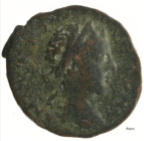
\includegraphics[width=.1\textwidth]{bilder/datenbanken_bsp1MA.jpg}};
		\node[right=0cm of fotoBspR]{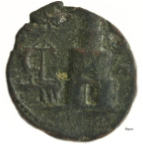
\includegraphics[width=.1\textwidth]{bilder/datenbanken_bsp1MR.jpg}};
		
		\draw[->, pfeil, semithick, shorten <=0em, shorten >=-0.4em] (fo-9Bsp.east) -- (muenzeBsp.west);
		\draw[->, pfeil, semithick, shorten <=0em, shorten >=-0.4em] (m-8Bsp.west) -- (fundortBsp.east);
		\draw[->, pfeil, semithick, shorten <=0em, shorten >=-0.4em] (m-9Bsp.east) -- (fotoBspA.west);
		\draw[->, pfeil, semithick, shorten <=0em, shorten >=-0.4em] (m-9Bsp.east) -- (fotoBspR.west);
		\draw[->, pfeil, semithick, shorten <=0em, shorten >=-0.4em] (fA-9Bsp.west) -- (muenzeBsp);
		\draw[->, pfeil, semithick, shorten <=0em, shorten >=-0.4em] (fR-9Bsp.west) -- (muenzeBsp.east);

		\node[below left=0.5cm and -4.3cm of fundortBsp]{Darstellung mit Beispieldaten};
	\end{tikzpicture}
	}%	
	
	\end{center}
	\caption{Beispiel einer objektorientierten Datenbank anhand von Münzdaten}
	\label{abb:datenbanken-objektorientiert}
\end{figure}


{\bfseries NoSQL Datenmodell:} Der Begriff NoSQL steht für "`Nicht nur SQL"' (Not only SQL) und bezeichnet Datenbanken, welche kein relationales Datenschema, sondern andere Paradigmen verfolgen. Sie können in zwei Typen unterschieden werden:
\begin{itemize}
	\item Bei \textbf{dokumentenorientierten Datenbanken} wird die zusammengehörige Informationsmenge in einem einzelnen Dokument gespeichert. Die Daten werden in Feldname-Wert-Paaren (z. B. Datierung: Römisch) z.B. im JSON Format (Abbildung \ref{abb:datenbanken-nosql}) gespeichert, wobei nicht jedes Paar vorhanden sein muss, was eine gewisse Flexibilität erlaubt.
	\item \textbf{Graphen-Datenbanken} können als moderne Nachfolger von Netzwerkdatenbanken verstanden werden, die vor allem bei sehr stark vernetzten Daten verwendet werden. Auch hier werden mit Hilfe von Graphen die Daten als Knoten dargestellt und die Beziehungen zwischen Ihnen als Kanten, wobei sowohl die Knoten als auch die Kanten Eigenschaften besitzen.
\end{itemize}

\begin{figure}[!htb]
\begin{center}
\lstset{language=HTML} %ist eigentlich JSON, aber die Optik von HTML passt auch
\begin{lstlisting}[frame=L, xleftmargin=0.3cm, rulecolor=\color{ianusGrau}, basicstyle=\footnotesize]
{
	"id":1,
	"Fundstellen_Name":"Korinth",
	"Breite"':37.91,
	"Länge"':22.87,
	"Münzen"'[
		{
			"id":23,
			"Münzen_Name":"Commodus aus Korinth",
			"Metall":"Bronze",
			"Fotos":[
				{
					"id":49,
					"Foto_Name":"Fundfoto -- Avers"
				},
				{
					"id":50,
					"Foto_Name":"Fundfoto -- Revers"
				}
			]
		},
		{
			"id":24,
			"Münzen_Name":"Münze aus Korinth",
			"Metall":"Bronze",
			"Fotos":[
				{
					"id":51,
					"Foto_Name":"Fundfoto"
				}
			]
		}
	]
}		
\end{lstlisting}
\end{center}
\caption{Beispiel einer NoSQL Datenbank im JSON Format anhand von Münzdaten}
\label{abb:datenbanken-nosql}
\end{figure}

\subparagraph{Relationale Datenbanken}
Das relationale Datenmodell hat sich als Standard von Datenbankanwendungen etabliert, da sich damit die Realwelt mit recht einfachen und realitätsnahen Strukturen abbilden lässt. In der archäologischen Forschung wird dieses Datenmodell fast ausschließlich eingesetzt.

Vereinfacht kann man sich eine relationale Datenbank als eine Sammlung von Tabellen (Relationen) vorstellen, in denen jeder Datensatz in einer Zeile (Tupel) einer Tabelle gespeichert wird (Abbildung \ref{abb:datenbanken-relation}). Jede Zeile besteht aus einer Anzahl von Attributen (Eigenschaften), den Spalten der Tabelle. Jedes Attribut hat einen eindeutigen zur Referenzierung dienenden Namen und einen bestimmten Attributtyp, welcher definiert welche Art von Daten -- beispielsweise Zeichensätze (String) oder Fließkommazahlen (Float) -- in dem Attribut gespeichert werden können. Jedes Attribut kann Werte entsprechend ihres Wertebereiches aufnehmen, der sich aus den Attributtyp ergibt. Zum Beispiel kann eine Münze mit Hilfe folgender Attribute (mitsamt Attributtypen) beschrieben werden: ID (Integer), Nominal (String), Datierung (String), Material (String), Durchmesser (Integer), Gewicht (Float), Funddatum (Date). 

\begin{figure}[h!tb]
\begin{center}
\scriptsize
\resizebox{1\textwidth}{!}{%
	\begin{tabular}{!\tbg  c!\tbg c!\tbg c!\tbg c!\tbg c!\tbg c!\tbg c!\tbg l}
		\arrayrulecolor{ianusGrau}
		\multicolumn{7}{c}{Attribute (Spalten)} &  \\
		\multicolumn{7}{c}{\color{ianusBlau} $\overbrace{\rule{9cm}{0pt}}$} & \\
		\cline{1-7}
		\cellcolor{BrickRed!10}ID & \cellcolor{BrickRed!10}Nominal & \cellcolor{BrickRed!10}Datierung & \cellcolor{BrickRed!10}Material  & \cellcolor{BrickRed!10}Dm. & \cellcolor{BrickRed!10}Gew. & \cellcolor{BrickRed!10}Funddatum & \hspace{-0.15cm}{\color{BrickRed}\textbf{--}Relationen-Schema} \\ 
		\cline{1-7}
		1 & Sesterz & römisch & Bronze & 36 & 28,68 & 25.02.1993 & \\
		\cline{1-7}
		2 & Tetradrachme & römisch & Gold & 25 & 13 & 13.08.2008 &\\
		\cline{1-7}
		\cellcolor{ianusBlau!10}3 & \cellcolor{ianusBlau!10}Tessera & \cellcolor{ianusBlau!10}römisch & \cellcolor{ianusBlau!10}Silber & \cellcolor{ianusBlau!10}18 & \cellcolor{ianusBlau!10}2,5 & \cellcolor{ianusBlau!10}12.02.1932 & \hspace{-0.15cm}{\color{ianusBlau}\textbf{--}Tupel (Datensatz)} \\
		\cline{1-7}
		4 & Drachme & griechisch & Silber & 27 & 5,68 & 12.03.2012 &\\
		\cline{1-7}
	\end{tabular}
}%	
\end{center}
  \caption{Aufbau der Relation "`Münze"' am Beispiel von Informationen zu Münzen.}
\label{abb:datenbanken-relation}
\end{figure}

Pro Tabelle werden immer nur gleichartige, reale Objekte (Entitäten) erfasst, z. B. nur Befunde, nur Münzen, nur Fotos, nur Bauwerke etc. Die eindeutige Referenzierung eines Datensatzes erfolgt mit Hilfe eines oder mehrer Schlüsselattribute, dem sogenannten Primärschlüssel. Dieser Schlüssel ist einzigartig und darf sich niemals ändern, da damit die Zeile in der Tabelle referenziert wird. Der Aufbau aller Tabellen, die zu einer Datenbank gehören, also die Datenbankstruktur, muss in dem Datenkatalog dokumentiert werden. Dieser enthält somit alle Festlegungen und Detailinformationen, die die Struktur der Datenbankinhalte in einem konkreten DBMS beschreiben, z.B. den Typ verschiedener Attribute (Kurztext, Langtext, Zahlen, Datum, Medien, etc.) und die Abhängigkeiten der Attribute zueinander. Der wichtigste Teilaspekt des Datenkataloges ist das Datenbankschema, das in abstrahierter Form die Beziehung und Art der Speicherung von Einzelinformationen festlegt.


\subparagraph{Beziehungen}
Einzelne Tabellen können anhand von Schlüsseln miteinander in Beziehung gesetzt werden, um Beziehungen zwischen einzelnen Datensätzen aus den unterschiedlichen Tabellen explizit auszudrücken. Beispielsweise um einer Münze, welche in der Tabelle "`Münze"' gespeichert ist, einem Fundort, welcher in der Tabelle "`Fundort"' gespeichert ist, zuzuweisen (Abbildung \ref{abb:datenbanken-beziehung}). Mit Hilfe von Primärschlüsseln (Hauptschlüssel, engl. Primary Key) wird der Datensatz einer Relation eindeutig definiert, wie im vorliegenden Beispiel mit Hilfe des Attributs "`Muenze-ID"'. Der Primärschlüssel einer Relation darf dabei nur einmal vorkommen, muss also einzigartig sein, um eine Referenzierung zu gewährleisten.
 
Ein Fremdschlüssel (engl. Foreign Key) dient zur Referenzierung eines Primärschlüssels einer anderen Tabelle. In dem Münzenbeispiel wurde die Relation "`Muenze"' um eine Attribut "`FS\_FundortID"' erweitert. Es ist ein Fremdschlüssel, welcher auf den Primärschlüssel "`PS\_FundortID"' der Relation Fundort verweist.

\begin{figure}[h!tb]
\begin{center}
\scriptsize
\resizebox{1\textwidth}{!}{%
	\begin{tabular}{!\tbg  c!\tbg c!\tbg c!\tbg c!\tbg c!\tbg c!\tbg c!\tbg c!\tbg}
		\arrayrulecolor{ianusGrau}
		\cline{1-5}
		\cline{7-8}
		\cellcolor{ianusGrau!10}ID & \cellcolor{ianusGrau!10}Nominal & \cellcolor{ianusGrau!10}... & \cellcolor{ianusGrau!10}Funddatum & \cellcolor{ianusGrau!10}FS\_FundortID & {\color{ianusBlau} \textbf{$\leftrightarrow$}}& \cellcolor{ianusGrau!10}PS\_FundortID & \cellcolor{ianusGrau!10}Ortsname \\ 
		\cline{1-5}
		\cline{7-8}
		1 & Sesterz & ... & 25.02.1993 & \cellcolor{ForestGreen!10}2 & & \cellcolor{ianusBlau!10}1 & \cellcolor{ianusBlau!10}Paris \\
		\cline{1-5}
		\cline{7-8}
		2 & Tetradrachme & ... & 13.08.2008 & \cellcolor{ianusBlau!10}1 & & \cellcolor{ForestGreen!10}2 & \cellcolor{ForestGreen!10}Haifa \\
		\cline{1-5}
		\cline{7-8}
		3 & Tessera & ... & 12.02.1932 & \cellcolor{ianusBlau!10}1 & & 3 & Alexandria \\
		\cline{1-5}
		\cline{7-8}
		4 & Drachme & ... & 12.03.2012 & \cellcolor{BrickRed!10}4 & & \cellcolor{BrickRed!10}4 & \cellcolor{BrickRed!10}Athen\\
		\cline{1-5}
		\cline{7-8}
	\end{tabular}
}%
\end{center}
  \caption{Beispielhafte Beziehung zwischen der Relation "`Muenze"' und der Relation "`Fundort"'.}
\label{abb:datenbanken-beziehung}
\end{figure}


Die Beziehungen zwischen zwei verschiedenen Relationen können dabei mit den folgenden gebräuchlichen Beziehungstypen beschrieben werden. Der Beziehungstyp wird dabei mit Hilfe einer Mengenangabe, der Kardinalität, angesprochen, der angibt wie viele Datensätze einer Relation mit wie vielen Datensätzen einer weiteren Relation in Beziehung stehen:
\begin{itemize}
	\item In 1 : 1 - Beziehungen ist jedem Datensatz einer Tabelle A nur ein einziger passender Datensatz in Tabelle B zugeordnet. Diesen Beziehungstyp verwendet man unter anderem, um eine unübersichtliche Tabelle mit vielen Attributen in mehrere übersichtliche Tabellen aufzuteilen. Beispielsweise werden in einer Tabelle für Münzen allgemeine Eigenschaften abgebildet und die Einzelheiten für die Vorder- und Rückseite einer Münze werden in gesonderten verknüpften Tabellen beschrieben.
	\item In 1 : N - Beziehungen, können einem Datensatz der Tabelle A mehrere passende Datensätze aus Tabelle B zugeordnet sein, wobei jedoch einem Datensatz aus Tabelle B nie mehr als ein Datensatz aus Tabelle A zugeordnet werden kann. Beispielsweise können an einem Fundort mehrere Münzen gefunden worden sein, aber eine Münze kann nur einen Fundort haben, wie in der Abbildung oben dargestellt ist.
	\item Bei M : N - Beziehungen können jedem Datensatz aus einer Tabelle A mehrere passende Datensätze aus einer Tabelle B zugeordnet sein und umgekehrt. Auf einem Foto können beispielsweises mehrere Münzen zu sehen sein, während es für eine Münze auch mehrere Fotoansichten geben kann.
\end{itemize}

\subparagraph{Attributtypen}
Es gibt verschiedene Attributtypen, die spezifische Informationen und Wertebereiche speichern:
\begin{itemize}
	\item Ganze Zahlen (integer, long) sind zu verwenden für Schlüssel, ordinalskalierte Variablen, wie etwa Schulnoten, oder sonstige numerische Angaben, bei denen die Genauigkeit ganzer Zahlen ausreichend ist.
	\item Fließkommazahlen (float) kommen zum Beispiel bei metrischen Maßen zum Einsatz. Bei allen Maßeinheiten ist zu beachten, dass in der Attributdefinition die verwendete Maßeinheit notiert und diese während der Benutzung auch einheitlich verwendet wird.
	\item Bool'sche Felder lassen nur zwei Werte zu: "`ja"' (1) oder "`nein"' (0) bzw. "`wahr"' oder "`falsch"'.
	\item Textfelder (varchar) können mit einer maximalen Länge definiert werden oder aber ohne weitere Angaben standardmäßig bis maximal 255 Zeichen verwendet werden. 
	\item Größere Textfelder (text) erlauben einen beliebig langen Freitexteintrag. Sie sollten so wenig wie möglich verwendet werden, da sie verhindern Informationen strukturiert einzutragen und somit ein gezieltes Auffinden erschweren. Sie können bei einer späteren Konvertierung einer DB in ein neues System Schwierigkeiten verursachen.
	\item Medienfelder/Binary Large Objects (BLOBs) ist ein binärer Datentyp, der zur datenbankinternen Speicherung von externen Medieninhalten (Fotos, Zeichnungen, Filme, Texte etc.) verwendet werden kann. Jedoch empfiehlt es sich diese Medieninhalte außerhalb der eigentlichen Datenbank zu speichern und nur die Referenz auf den Speicherort der externen Ressource in einem Attribut zu erfassen. Dadurch werden u. a. die Datenbankgröße überschaubar gehalten, eine konsistente Datenhaltung der Einzeldaten gewährleistet und Probleme beim Export der Datenbankinhalte reduziert. Ist im Ausnahmefall dennoch das Importieren von externen Medieninhalten notwendig, sollten diese für den jeweiligen Zweck optimiert sein (z. B. sind für die Bildvorschau geringe Bildauflösungen ausreichend).
\end{itemize}

\subparagraph{Structured Query Language (SQL)}
Mit Hilfe von speziellen Datenbanksprachen kann ein Benutzer oder ein externes Programm über das DMBS mit einer Datenbank kommunizieren. Die am weitesten verbreitete Datenbanksprache im Bereich der relationalen Datenbanken ist SQL (structured query language). Sie wird rechnerunabhängig und produktübergreifend seit 1986 im ISO Standard 9075 definiert. Seitdem erfuhr SQL sieben Erweiterungen, von denen die letzte Aktualisierung 2011 als ISO/IEC 9075:2011 erschienen ist.

SQL-Befehle lassen sich in vier verschiedene Befehlsgruppen unterteilen (Tabelle \ref{tab:datenbanken-SQL}).

\begin{table}[hbt]
\lstset{
  language=SQL,
  basicstyle=\footnotesize,
	xleftmargin=-0.5cm,
	aboveskip=-0.2cm,
	belowskip=-0.2cm
  }
\centering
\footnotesize
\begin{tabular}{L{0.2\textwidth} p{0.3\textwidth} p{0.4\textwidth}}
	\toprule
	Befehlsgruppe	& Beschreibung & Beispiel \\
	\midrule
	Data Definition Language (DDL)	& Befehle zur Definition des Datenbankschemas: Erstellen von Datenbanken, Tabellen und Indizes. 
	& \begin{lstlisting}
		/* Anlegen der Tabelle 'muenzen'
		 mit beispielhaften Attributen 
		 unter Angabe des Datentyps */
		CREATE TABLE muenzen
		(PS_MuenzID serial NOT NULL,
			Nominal varchar,
			Gewicht float);
\end{lstlisting}
	\\
	Data Query Language (DQL) & Befehle zum Abfragen von Daten. & 
	\begin{lstlisting}
		/* Abfrage nach allen Münzen 
		 mit Fundort Paris */
		SELECT * 
		FROM muenzen
		WHERE FS_FundortID = '1'
	\end{lstlisting}
	\\
	Data Manipulation Language (DML) & Befehle zur Datenmanipulation, also dem Ändern, Bearbeiten und Löschen von Datensätzen. & 
	\begin{lstlisting}
		/* Ändern des Materials in 
		  Gold für den dritten Datensatz */
		UPDATE muenzen 
		SET Material = 'Gold' 
		WHERE PS_MuenzID = '3'
	\end{lstlisting} 
	\\
	Data Control Language (DCL) & Befehle zum Anlegen von Benutzern und zur Definition von Zugriffsrechten & 
	\begin{lstlisting} 
		-- Nutzer mit Passwort anlegen
		CREATE USER mmustermann
		PASSWORD 'passwort'
	\end{lstlisting}
	\\
	\bottomrule 
\end{tabular}
\caption{SQL-Befehle lassen sich in vier verschiedene Befehlsgruppen unterteilen}
\label{tab:datenbanken-SQL}
\end{table}

\subparagraph{Entity-Relationship-Modell (ERM)}
Ein wichtiges grafisches Hilfsmittel beim Entwurf und zur Dokumentation einer Datenbank ist das Entity-Relationship-Modell (ERM). Neben der grafischen Visualisierung mittels eines Entity"=Relationship"=Diagram (ERD) ist auch die tabellarische Erfassung und Beschreibung aller Entitätstypen, Beziehungstypen und Attribute für eine vollständige Dokumentation einer Datenbank notwendig. Das ERD ist ein beschriftetes Diagramm mit festgelegten Symbolen, das dazu dient, den gewünschten Ausschnitt der realen Welt formal zu beschreiben. Grundlage der ER"=Modelle ist die Abstraktion von Objekten und deren Beziehungen untereinander. Folgende grundlegende Begriffe in einem ERM und deren grafische Wiedergabe in einem ERD werden in diesem Zusammenhang unterschieden: (Tabelle \ref{tab:datenbanken-ERD}).

\begin{table}[h!bt]
\centering
\footnotesize
\begin{tabular}{L{0.15\textwidth} p{0.45\textwidth} C{0.3\textwidth}}
	\toprule
	Element	& Beschreibung & Grafische Darstellung \\
	\midrule
	Entität (Datensatz)	& Objekt der Wirklichkeit, materiell oder abstrakt, z. B. ein Fund "`Münze XY"', ein Befund "`Pfostenloch 123"' oder eine Abteilung "`DAI Rom"'. & keine grafische Darstellung \\
	Entitätstyp (Tabelle) & Abstraktion gleichartiger Entitäten, z. B. Personen, Funde, Befunde, Adressen.\vspace{0.3cm}& 
	\begin{tikzpicture}[baseline=0.1cm]
		\node[eckigeBox] {Muenze};
	\end{tikzpicture}%
	\\
	Beziehung & semantische Beziehung zwischen verschiedenen Datensätzen aus unterschiedlichen Tabellen, z. B. "`Münze"' in "`Pfostenloch"' & 
	\begin{tikzpicture}
		\node[raute] (kern) {};
		\node[left = 0.6cm of kern] (links) {};
		\node[right = 0.6cm of kern] (rechts) {};
		\path[linie] (kern) edge (links);
		\path[linie] (kern) edge (rechts);
	\end{tikzpicture}%
	\\
	Beziehungstyp & Abstraktion gleichartiger Beziehungen, z. B. "`gefunden in"'. & 
	\begin{tikzpicture}
		\node[raute] (kern) {\tiny gefunden in};
		\node[left = 0.6cm of kern] (links) {};
		\node[right = 0.6cm of kern] (rechts) {};
		\path[linie] (kern) edge (links);
		\path[linie] (kern) edge (rechts);
	\end{tikzpicture}%
	\\
	Kardinalität & mögliche Anzahl der an einer Beziehung beteiligten Entitäten (s. u. Beziehungsarten); Symbol: 1, N oder M über Strich & 
	\begin{tikzpicture}
		\node[raute] (kern) {};
		\node[left = 0.6cm of kern] (links) {};
		\node[right = 0.6cm of kern] (rechts) {};
		\path[linie] (kern) edge node [near end, label=above:1] {} (links);
		\path[linie] (kern) edge node [near end, label=above:n] {} (rechts);
	\end{tikzpicture}%
	\\
	Attribut & Eigenschaften eines Entitätstyps oder eines Beziehungstyps, z. B. Geburtsdatum von Personen. & 
	\begin{tikzpicture}[baseline=0.2cm]
		\node[ellipseDick] {Durchmesser};
	\end{tikzpicture}%
	\\
	Schlüssel & Attribut/e, welche/s zur eindeutigen Identifizierung einer Entität von einem Entitätstypen dient/en. & 
	\begin{tikzpicture}[baseline=0.2cm]
		\node[ellipseDick] {\underline{PS\_MuenzID}};
	\end{tikzpicture}%
	\\
	\bottomrule 
\end{tabular}
\caption{Grundlegende Begriffe in einem ERM und deren grafische Wiedergabe in einem ERD.}
\label{tab:datenbanken-ERD}
\end{table}

\subparagraph{Bestandteile einer Datenbank}
Um eine Datenbank auch zukünftig nutzen und die in ihr erfassten Inhalte verstehen zu können, ist eine umfassende und vollständige Dokumentation erforderlich, zu der verschiedene Komponenten gehören:
\begin{itemize}
	\item Die schriftliche und/oder tabellarische Anforderungsanalyse
	\item Die eigentlichen Datenbankinhalte
	\item Die Beschreibung der Datenstruktur
	\item Die Definition der implementierten Funktionalitäten
	\item Semantisch-inhaltliche Aspekte wir vorgegebene Wertelisten, Thesauri oder individuelle Definitionen von Begriffen und Datensätzen
	\item Dokumentation der grafischen Benutzeroberflächen und verschiedenen Sichten auf die Daten (z.B. Eingabeformulare, Suchmasken, Ausgabeformate), technischen Schnittstellen und  erstellten Regelwerke (z.B. Benutzerhandbücher) 
\end{itemize}

Da mit keinem der empfohlenen Dateiformate alle Komponeneten erfasst und archiviert werden können, ist eine hybride Archivierungsstrategie erforderlich. Beispielsweise können der Inhalt, die Struktur und die Funktionalitäten einer Datenbank im SIARD-Format archiviert werden. Die Anforderungen werden schriftlich beschrieben und um ein grafisches Enitity-Relationship-Diagramm ergänzt. Individuelle Vorgaben zur Benutzung (insbesondere der Dateneingabe) werden mittels eines Benutzerhandbuches im Format PDF/A dokumentiert und die einzelnen Layoutmasken werden mittels Screenshots als unkomprimierte TIFF-Dateien gespeichert.

Die folgenden Tabelle gibt einen Überblick über die verschiedenen Formate für Datenbanken und welche davon für die langfristige Speicherung der genannten Dokumentationskomponenten  von Datenbanken geeignet sind.

\begin{table}[hbt]
\centering
\footnotesize
\begin{tabular}{R{0.4\textwidth} cccc}
	\toprule
	Format, Dokument	& I & S & F & B \\
	\midrule
	SIARD & \checkmark & \checkmark & \checkmark & \\
	SQL & \checkmark & \checkmark & \checkmark &  \\
	XML & \checkmark & (\checkmark) &  &  \\
	CSV & \checkmark & & & \\
	JSON & \checkmark & & & \\
	\midrule
	ERD (z. B. TIFF) & & & \checkmark &  \\
	Benutzerhandbuch (z. B. PDF/A) & & & & \checkmark \\
	beschriebene Bildschirmfotos (z. B. TIFF) & & & &  (\checkmark)\\
	\midrule
	MDB, ACCDB & & & &  \\
	FP5, FP7, FMP12 & & & &  \\
	ODB & & & & (\checkmark) \\
	DMP, BAK, DB & & & &  \\
	\bottomrule 
\end{tabular}
\caption{Formate für Datenbanken und welche Elemente sie langfristig Speichern können. I~= Datenbankinhalt, S~=Datenbankstruktur, F~= Funktionalitäten, B~=Benutzung. Leere Zellen bedeuten fehlende Speichereigenschaften.}
\label{tab:datenbanken-Eigenschaften}
\end{table}


%########################################################################

\paragraph{Praxis}
Für den praktischen Umgang mit Datenbanken werden Hinweise gegeben, die einerseits Aspekte, die schon bei dem Entwurf der Datenbank berücksichtigt werden sollten, andererseits aber auch Empfehlungen für die tägliche Arbeit mit einer Datenbank thematisieren, wie etwa Dateneingabe, Exportmöglichkeiten, Speicherung und Sicherung sowie mehrsprachige Dateneingabe.

Es werden verschiedene DBMS und Administratorentools vorgestellt, mit denen sowohl Desktop- als auch serverbasierte Datenbanken erstellt und betrieben werden können. Für die Archivierung von Datenbanken werden Programme zur automatischen Analyse und Dokumentation der Datenbankstruktur vorgestellt. Auch für die Speicherung in SIARD und den Umgang mit diesem Format gibt es ein eigenes Toolkit. Für FileMaker- und MSAccess-Datenbanken gibt es gesonderte Hinweise.

\subparagraph{Datenbankentwurf}
Der Datenbankentwurf bzw. das Datenbankschema hat einen großen Einfluss auf die  Qualität einer Datenbank. Die richtige Strukturierung von Informationen vor der eigentlichen Eingabe von Daten stellt die Voraussetzung für eine langfristige, flexible und sinnvolle Verwendung einer Datenbank dar -- vor allem dann, wenn sich im Laufe der Zeit die Anforderungen und Wünsche ändern

Der Entwurf von Datenbanken erfolgt idealerweise in folgenden Schritten:
\begin{itemize}
	\item Anforderungsanalyse: Allgemeine Beschreibung des zukünftigen Systems in Rücksprache mit den Endanwendern, Sammlung der wissenschaftlichen und technischen Anforderungen, Definition der Eigenschaften der zu verarbeitenden Informationen, Festlegung der Arbeitsweise und Rechte der Benutzer, Einbindung von "`Altbeständen"' (alte Dokumentation, etc.) und Analyse der Häufigkeit verschiedener Abfragen und Eingaben.
	\item Konzeptueller Entwurf: Erstellung eines softwareunabhängigen Datenbankschemas, welches sich als globale Sicht auf die Daten aus den Einzelsichten der jeweiligen Nutzergruppen zusammensetzt. Hierfür empfiehlt sich eine grafische Darstellung, z. B. als Entity-Relationship-Diagramm (ERD). 
	\item Logischer Entwurf: Umsetzung des konzeptuellen Entwurfs auf ein gewähltes DBMS, z. B. durch Übertragung des ERD in einen Datenkatalog.
	\item Datendefinition: Konkrete Realisierung des logischen Entwurfs in einem DBMS, z.B. indem die im Datenkatalog festgelegten Spezifikationen in einer Datenbank-Software angelegt und gespeichert werden.
	\item Benutzerrechte: Festlegung, welcher Benutzer welche Daten in welcher Form sehen, bearbeiten, löschen, exportieren, drucken etc. darf.
	\item Dokumentation: Strukturiertes Festhalten des Datenbankentwurfes, der Attributdefinitionen, zulässiger Werte, Indizes, Layouts etc. und der dahinter stehenden Überlegungen. 
\end{itemize}

Bei der Entscheidung, welche Eigenschaften eines realen Objektes durch welche Attribute einer Entität beschrieben werden, sollten folgende Punkte beachtet werden: Grundsätzlich sind die Eigenschaften (Attribute) eines Entitätstypes möglichst klein bzw. atomar zu halten (z. B. statt einem Attribut "`Maßangaben"' sind verschiedene Attribute wie "`Höhe"', "`Breite"', "`Tiefe"' etc. sinnvoller). Dies erleichtert präzise Abfragen und Berechnungen sowie den späteren Austausch der Daten mit anderen Systemen. Eine automatische Zusammenführung von Daten aus mehreren atomaren Attributen in ein einziges, umfangreicheres Attribut  ist immer möglich -- der umgekehrte Weg, also eine automatische Aufteilung eines größeren Attributes auf viele kleinere, dagegen meist nicht. Dabei sollte bedacht werden, dass die Bearbeitungszeit eines Datensatzes mit der Anzahl der auszufüllenden Attribute wächst. Je nach Fragestellung und Anforderung muss ein ausgewogenes Verhältnis von Datenvielfalt (Vollständigkeit) und Effizienz gefunden werden.

Es wird dringend empfohlen, dass ein Datenbankentwurf vor dessen praktischer Umsetzung von einem Fachmann zur Informationsmodellierung nach inhaltlichen und formalen Kriterien (z. B. hinsichtlich Inkonsistenzen, Integritätsbedingungen, Redundanzen, Möglichkeiten der Verbesserung etc.) überprüft wird. In diesem Austausch sollte dann auch diskutiert werden, inwieweit ein vorhandenes Schema in die sog. erste bis fünfte Normalformen überführt werden kann oder nicht. Bei diesem Prozess der Normalisierung handelt es sich um ein in der Informatik entwickeltes Konzept zur Vermeidung von Anomalien der Datenbankinhalte und zur Beurteilung der Qualität eines relationalen Datenbankschemas, das allerdings ein vertieftes Verständnis zur Funktionsweise von DBMS voraussetzt.

\subparagraph{DBMS für Desktop-Datenbanken}
Allen Desktop"=Datenbankmanagementsystemen ist gemeinsam, dass eine gleichzeitige Nutzung durch mehrere Benutzer nur unzureichend möglich ist, weswegen diese nur für kleinere bis mittlere Datenbanken im lokalen Betrieb empfohlen werden können. In der Regel besteht auch die Möglichkeit ein Desktop-DBMS in einer Hybridlösung als Frontend zur Dateneingabe zu verwenden, während die Datenhaltung in einem serverbasierten DBMS erfolgt.

Sofern die Anforderung besteht, eine Datenbank für mehrere Benutzer betreiben zu wollen, sollte auf jeden Fall die Verwendung eines DBMS für eine Server-Datenbank in Betracht gezogen werden. Kann eine Server-Client-Architektur für mehrere Benutzer nicht realisiert werden und wird stattdessen parallel mit mehreren Desktop-Datenbanken gearbeitet, müssen gesonderte Vorkehrungen bei der Entwicklung der Datenbank getroffen werden und deren strikte Einhaltung gewährleistet werden, damit die Datenbankinhalte trotzdem konsistent bleiben (z. B. Vergabe individueller Nummernblöcke für einzelne Bearbeiter; Einschränkungen durch ein detailliertes Rechte-Management; regelmäßige Datenzusammenführungen, um frühzeitig Inkonsistenzen und Widersprüche im Datenbestand festzustellen).

{\bfseries FileMaker Pro} ist ein kommerzielles DBMS für die Betriebssysteme Mac OS und Windows, das sich neben Microsoft Access zum Standardprogramm für Datenbanken auf Einzelplatzrechnern entwickelt hat. Charakteristisch ist seine einfache Benutzbarkeit, die es ermöglicht schnell Lösungen zu realisieren. Der Export der Datensätze in Standardformate (z. B. CSV, XML, XLS) ist gewährleistet, der Export der Datenbankstruktur ist mit FileMaker Advanced in den Formaten HTML oder XML möglich. Es gibt jedoch auch einige Schwächen wie die mangelnde Unterstützung von SQL und von Geodaten, erhöhte Anschaffungskosten und das Fehlen einer echten Programmiersprache.

{\bfseries Microsoft Access} ist Bestandteil des Office-Professional-Pakets von Microsoft, das nur für das Windows-Betriebssystem angeboten wird. Alle Datenbankelemente, inkl. aller Elemente der Oberflächen als auch die Datenbanktabellen selbst, werden in einer einzigen Datei des proprietären MDB- bzw. ACCDB-Dateiformates abgespeichert. MS Access bietet im Vergleich zu FileMaker Pro weniger unterstützte Macros an, so dass umfangreiche Funktionen mit der Programmiersprache Visual Basic selbst entwickelt werden müssen. Dadurch können auch komplexe Aufgaben erstellt und individuelle Anpassungen vorgenommen werden, was bei FileMaker Pro mit den internen Script-Möglichkeiten nur eingeschränkt möglich ist. Nachteilig sind u.a. die Größenbegrenzung auf 2 GB und eine Instabilität bei größeren Anwendungen.

{\bfseries OpenOffice Base} ist ein DBMS, welches im Office Paket von OpenOffice bzw. LibreOffice enthalten ist. Das in der Programmiersprache Java entwickelt Programm steht als Open Source zur Verfügung und kann daher ohne zusätzliche Kosten auf vielen unterschiedlichen Betriebssysteme installiert werden. Das Backend von Base wird mit Hilfe der sehr stabilen und robusten Datenbank HSQLDB betrieben, wobei das DBMS jedoch auch viele verschiedene Datenbanktreiber und Schnittstellen unterstützt. Gegenüber den kommerziellen Lösungen ist die Gestaltung der Oberflächen umständlicher und weniger umfangreich.

{\bfseries SQLite} ist das weltweit am häufigsten verwendete DBMS, da es im Bereich von Android Smartphones und Browsern zum Speichern von Daten verwendet wird. Die Daten werden in einer einzigen SQLite Datenbank gespeichert. Mit Hilfe der GIS Erweiterung SpatiaLite lassen sich auch Geodaten verarbeiten. Es existiert keine Client-Server Architektur, weswegen das DBMS nur von einem Einzelbenutzer betrieben werden sollte.

\begin{flushleft}
FileMaker Pro: \urllist{http://www.filemaker.com/}
Microsoft Access: \urllist{https://products.office.com/de-DE/access}
OpenOffice Base: \urllist{https://www.openoffice.org/product/base.html}
SQLite: \urllist{https://sqlite.org/}
\end{flushleft}


\subparagraph{DBMS für Server-Datenbanken}
Serverbasierte Datenbankmanagementsysteme bilden die Grundlage für Datenbanken, die kollaborativ und webbasiert, z.B. über einen Internet-Browser, genutzt werden sollen. Anders als DBMS für Desktop-Datenbanken werden keine weiteren Möglichkeiten zur Gestaltung von grafischen Oberflächen (z.B. Eingabeformulare oder Listendarstellungen) bereitgestellt. Diese müssen mit Hilfe von Programmiersprachen (z.B. JavaScript, PHP oder Java) erstellt werden, was fundierte Software- und Informatikkenntnisse zur Entwicklung von Datenbankanwendungen voraussetzt. Insofern sind sie als Systeme für "`schnelle Lösungen"' ungeeignet, da in der Regel ein längerer Planungs- und Entwicklungszeitraum benötigt wird. 

Gegenüber Desktop-Datenbanken, die u.U. parallel und technisch unabhängig voneinander betrieben werden, besitzen sie jedoch erhebliche Vorteile hinsichtlich einer konsistenten Datenhaltung. Der Betrieb eines Server DBMS in einer sogenannten Server-Client-Architektur ermöglicht es mehreren Benutzern, gleichzeitig auf den jeweils aktuellsten Datenbestand zuzugreifen. Bei einer parallelen Eingabe von Daten verschiedener Nutzer im selben Datensatz verhindert das DBMS, dass es zu Versionierungskonflikten oder Verletzungen von Integritätsbedingungen kommt und der Datenbestand inkonsistent wird.

{\bfseries MySQL und PostgreSQL} sind weit verbreitete kostenlose Open-Source-DBMS, die sich in ihrem Funktionsumfang stark ähneln. Der wesentliche Unterschied ist, dass PostgreSQL mit der Erweiterung PostGIS in der Lage ist, geografische Daten adäquat zu speichern und zu verarbeiten, was für die Auswertung der Datenbankinhalte in einem Geografischen Informationssystem (GIS) entscheidend ist. Daneben besitzt PostgreSQL gegenüber MySQL eine höhere Konformität zum SQL-Standard, unterstützt JSON-Objekte, hat bessere Methoden zur Wahrung der Datenintegrität und umfangreichere Möglichkeiten zur Erstellung von internen Funktionen (sog. Stored Prozedures). Jedoch weist MySQL durch seine weitere Verbreitung eine höhere Unterstützung von Web Frameworks auf. Für Datenbankanwendungen in der Archäologie kann insbesondere PostgreSQL empfohlen werden. Ein umfangreicher Vergleich beider Systeme kann als Auswahlhilfe dienen. Für den Entwurf eines DMBS in MYSQL kann das frei verfügbare Tool DBDesigner 4 verwendet werden. 

{\bfseries Microsoft SQL Server und Oracle} sind kommerzielle, serverbasierte DBMS mit einem vergleichbaren Funktionsumfang. Im direkten Vergleich ist Microsoft SQL Server einfacher zu administrieren und billiger in den Anschaffungskosten, während Oracle die umfangreichsten Erweiterungs- und Anpassungsmöglichkeiten bietet, welche jedoch kaum einen praktischen Mehrwert für Datenbanken in den digitalen Geisteswissenschaften besitzen.

\begin{flushleft}
MySQL: \urllist{https://www.mysql.com/}
PostgreSQL: \urllist{https://www.postgresql.org/}
Vergleich von MySQL, PostgreSQL und SSLite: \urllist{https://www.digitalocean.com/community/tutorials/sqlite-vs-mysql-vs-postgresql-a-comparison-of-relational-database-management-systems}
Microsoft SQL Server: \urllist{https://www.microsoft.com/en-us/sql-server/sql-server-2016}
Oracle: \urllist{https://www.oracle.com/database/index.html}
DBDesigner 4: \urllist{http://fabforce.eu/dbdesigner4/}
\end{flushleft}


\subparagraph{Administration von Server-Datenbanken}
Für alle genannten DBMS für Server-Datenbanken existieren grafische Administrationstools, mit deren Hilfe Anfragen an die Datenbank generiert werden können. Sie lassen sich nach Desktop- und webbasierten Anwendungen unterschieden sowie nach der Anzahl der unterstützten DBMS, da einige Tools entweder nur für ein spezifisches oder aber generisch für verschiedene DBMS geeignet sind.

Zu den empfehlenswerten Desktopanwendungen gehören die Tools pgAdmin3 (für PostgreSQL), MySQL Workbench (für MySQL), SQLite Database Browser (für SQLite), Oracle SQL Developer (für Oracle), SQL Server Management Studio (für Microsoft SQL Server) und SQuirrel SQL (u.a. für PostgreSQL, MySQL, Oracle, MicrosoftSQL, Microsoft Access). Webbasierte Administrationstools sind beispielsweise phpmyadmin (für MySQL), phppgadmin (für PostgreSQL) oder Adminer (für MySQL, PostgreSQL, SQLite, MS SQL und Oracle).

\begin{flushleft}
pgAdmin3: \urllist{https://www.pgadmin.org/}
MySQL Workbench: \urllist{http://www.mysql.de/products/workbench/}
SQLite Database Browser: \urllist{http://sqlitebrowser.org/}
Oracle SQL Developer: \urllist{http://www.oracle.com/technetwork/developer-tools/sql-developer/}
SQL Server Management Studio: \urllist{https://msdn.microsoft.com/de-de/library/mt238290.aspx}
SQuirrel SQL: \urllist{http://squirrel-sql.sourceforge.net/}
phpmyadmin: \urllist{https://www.phpmyadmin.net/}
phppgadmin: \urllist{http://phppgadmin.sourceforge.net/}
Adminer: \urllist{https://www.adminer.org/}
\end{flushleft}

\subparagraph{Dateneingabe und Datenqualität}
Zentral für den Nutzen einer Datenbank ist, dass die semantische Definitionen jeder Entität, und jedes Attributes bekannt sind, d.h. den einzelnen Bearbeitern muss bewusst sein, welche Eigenschaften eines Objektes der realen Welt in welchem Eingabefeld gespeichert werden. Dies kann entweder durch eine externe Dokumentation, deskriptive Eingabeformulare (z.B. mittels Hilfefunktionen), Beispieldatensätze, vorgegebene Termini (z.B. Werte-/Codelisten, Thesauri, Vokabulare) oder technische Funktionen (z.B. Indizes, Autovervollständigungen) unterstützt werden. Innerhalb eines Projektes individuell definierte oder extern importierte Wörter und Begriffe sollten bereits im Verlauf des Datenbankentwurfs festgelegt werden, um eine semantisch saubere Trennung verschiedener Attribute zu gewährleisten.

Von Anfang an und insbesondere bei Mehrbenutzersystemen muss auf eine einheitliche Verwendung von Begriffen und eine möglichst vereinheitlichte Eingabe der einzelnen Werte geachtet werden. So sollte z. B. die gleiche Ansprache von Ortsnamen entweder abgesprochen und dokumentiert werden, durch einen entsprechenden Datenbankentwurf kontrolliert werden oder -- im besten Falle -- durch referenzierte Vokabular und Normdaten gewährleistet werden. Andernfalls kann es durch unterschiedliche Schreibweisen und Rechtschreibfehler beim Wiederauffinden von an sich gleichen Inhalten zu Problemen kommen. Hilfreich zur Verbesserung der Datenqualität sind Index-Funktionen, die viele DBMS anbieten, da mit ihnen in der Regel schnell erfasst werden kann, welche Werte bereits in ein Attribut eingetragen wurden, und dadurch fehlerhafte Einträge leicht identifiziert werden können.

Bei metrischen Eingaben muss frühzeitig die spätere Auswertung (z.B. statistische oder räumliche Analysen) im Auge behalten werden, da diese die Speicherung als numerische Datentypen, die einheitliche Verwendung einer Maßeinheit, die als Metadatum in der Attributbeschreibung hinterlegt werden sollte, oder den Umgang mit unscharfen bzw. unvollständigen Werten beeinflusst.

Um möglichst vollständige Suchergebnisse zu erhalten und eine höhere Vergleichbarkeit der eingegebenen Daten zu gewährleisten, kann es sinnvoll sein, bei Eigenschaften von Entitäten, die als Freitext-Attribute modelliert werden (z.B. ausführliche Beschreibungen), zusätzlich ein inhaltlich äquivalentes Attribut mit kontrolliertem Vokabular vorzusehen (z.B. Schlagworte, die zu der freien Beschreibung passen). Bei längeren Freitext-Attributen ist es zudem ratsam, eine inhaltliche Strukturierung vorzugeben, oder es sollte überlegt werden, diese Informationen auf mehrere separate Attribute aufzuteilen.

Wenn ein Attribut nicht ausgefüllt ist, kann es in manchen DBMS einen sog. NULL-Wert annehmen. Dieser entspricht keinem Datentyp und ist nicht mit der numerischen Ziffer 0 gleichzusetzen. Es ist ein symbolischer Wert, der aussagt, dass kein Wert vorhanden ist. Da in solchen Fällen jedoch üblicherweise unklar ist, ob das Feld vergessen, übersehen, nicht verstanden wurde, keine Angabe vorliegt oder erst später bearbeitet werden soll (sog. Nullwert-Problematik), kann eine Eingabe erfolgen, die diese Unklarheit beseitigt. Dafür können etwa bestimmte Zeichen reserviert werden, die sich von jedem anderen Wert in einer Datenbank unterscheiden, z.B.:
\begin{itemize}
	\item Information zur Zeit unbekannt bzw. nicht relevant: NULL
	\item Information wird später nachgetragen: \#
	\item Aussage derzeit nicht eindeutig möglich oder zu beantworten: ?
\end{itemize}


\subparagraph{Schnittstellen und Exportmöglichkeiten}
Dient eine Datenbank u. a. als Arbeitsmittel zur strukturierten Erfassung von Daten, die in anderen Programmen weiterverarbeitet werden sollen, ist auf geeignete Exportformate zu achten. Oftmals kann die Entscheidung für oder gegen ein DBMS davon abhängen, wie gut oder schlecht die Datenbankinhalte aus dem ursprünglichen System wieder herausgeholt und nachgenutzt werden können; ein Aspekt der insbesondere für die Langzeitarchivierung von besonders hoher Relevanz ist. Prinzipiell lassen sich drei Arten von Exportmöglichkeiten unterscheiden, die von den allermeisten DBMS unterstützt werden:
\begin{itemize}
	\item Export einfacher textbasierter Dateiformate wie CSV oder TSV 
	\item Export komplexer strukturierter Dateiformate wie XML und JSON
	\item ODBC (Open Database Connectivity) und JDBC (Java Database Connectivity) sind universelle Schnittstellen, welche den Zugriff auf und den Datenaustausch mit einer Datenbank ermöglichen.
\end{itemize}


\subparagraph{Speicherung und Sicherung}
Da Datenbanken in den Altertumswissenschaften in der Regel statische Daten enthalten, die nach der initialen Eingabe und ggf. einer ersten Änderung kaum weiter modifiziert werden, sollte das Löschen von Datensätzen durch Sicherheitsabfragen und restriktive Zugriffsrechte abgesichert werden. Alle Veränderungen an dem Datenbankinhalt werden in der Regel immer sofort und ohne Interaktion mit dem Benutzer durch ein DBMS gespeichert. Dies hat den Vorteile, dass ein ’manuelles’ Speichern entfällt, aber auch den Nachteile, dass alle Dateneingaben -- also auch versehentlich falsche -- sofort gültig und ohne eine Sicherung vorheriger Zustände nicht revidierbar sind. Daher ist das Anlegen von Sicherungskopien oder Datenexporten, insbesondere vor größeren Veränderungen des Datenbestandes, sehr zu empfehlen. Alternativ kann mit Hilfe einer Versionierung, die jegliche Zustände der Datenbankinhalte abspeichert und vor allem bei Server-DBMS gut konfiguriert werden kann, auch auf ältere Stände zurückgegriffen werden.

\subparagraph{Mehrsprachigkeit}
Vor allem in internationalen Projekten besteht häufig die Anforderung, die Inhalte einer Datenbank mehrsprachig zu erfassen und auszuwerten. Eine technisch saubere Lösung, die die Inhalte in den verschiedenen Sprachen konsistent hält, ist nur mit relativ hohem Aufwand zu realisieren und muss sorgfältig geplant werden. Der Grad der Komplexität der Umsetzung hängt dabei auch davon ab, ob die Datenbank nur eine geringe und feste Anzahl von Sprachen (etwa nur zwei oder drei) oder prinzipiell beliebig viele unterstützen muss. Auf jeden Fall wirkt sich diese Anforderung auf den konzeptuellen und logischen Entwurf des Datenbankschemas aus.

Am einfachsten und unproblematischsten ist die Beschriftung der Benutzeroberflächen und Formulare (z. B. Überschriften, Bezeichnungen neben den Eingabefeldern, Hilfetexte) in verschiedenen Sprachen, da diese Elemente sich nicht auf die Datenbankinhalte selbst auswirken. Bei Attributen mit kontrolliertem Vokabular ist eine weitgehend automatische Übertragung in eine andere Sprache prinzipiell möglich, sofern Konkordanzlisten vorliegen. In diesen Fällen bietet sich die Benutzung internationaler Referenzsysteme an, bei denen Begriffe und Fachtermini bereits in verschiedenen Sprachen verwaltet werden, sowie im Wesentlichen auf abstrakte Konzepte -- unabhängig von ihren sprachlich unterschiedlichen Bezeichnungen -- verwiesen wird und die konkreten Wörter erst nach Auswahl einer Sprache durch den Datenbanknutzer nachgeladen werden. 

Am schwierigsten und zeitaufwendigsten ist die Behandlung von mehrsprachigen Freitextfeldern. Entweder muss in diesem Fall für eine Eigenschaft eines Objektes mehrere sprachspezifische Attribute definiert werden (beispielsweise Beschreibung-deu, Beschreibung-eng) oder aber die Eingabe muss mit Hilfe von Hinweistexten, sogenannten Tags, annotiert werde (z.B. \emph{$<$de$>$Der Avers zeigt den bekränzten Kopf von Nero nach rechts.$<$/de$>$ $<$en$>$The Avers shows the wreath head of Nero facing to the right.$<$/en$>$}) In beiden Varianten kann allerdings nicht gewährleistet werden, dass die Eingabe in der einen Sprache inhaltlich mit der Eingabe in der anderen Sprache tatsächlich übereinstimmt, was nur durch zusätzliche manuelle Kontrollen überprüft werden kann.


\subparagraph{Automatische Dokumentation der Datenbankstruktur}
Die Erfassung von Metadaten zu einer Datenbank kann je ihrer Komplexität sehr aufwendig sein, wobei sich verschiedene Tools zur automatischen Dokumentation der Datenbankstruktur anbieten, von denen besonders das Tool SchemaSpy zu empfehlen ist. Neben der Möglichkeit, Befehle direkt über eine Kommandozeile einzugeben, existiert mit SchemaSpyGUI auch eine grafische Benutzeroberfläche (Abbildung \ref{abb:datenbanken-SchemaSpyGUI} und \ref{abb:datenbanken-schemaspydoku}). 

\begin{figure}[!hbtp]
  \begin{center}
    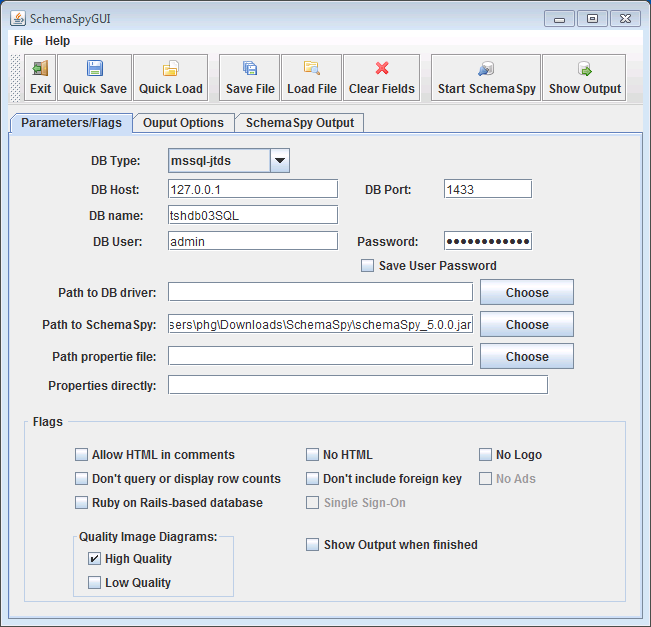
\includegraphics[width=0.7\textwidth]{bilder/datenbanken_SchemaSpy_GUI}
  \end{center}
  \caption{SchemaSpyGUI Benutzeroberfläche zur automatischen Dokumentation der Datenbankstruktur}
  \label{abb:datenbanken-SchemaSpyGUI}
\end{figure}

\begin{figure}[!hbtp]
  \begin{center}
    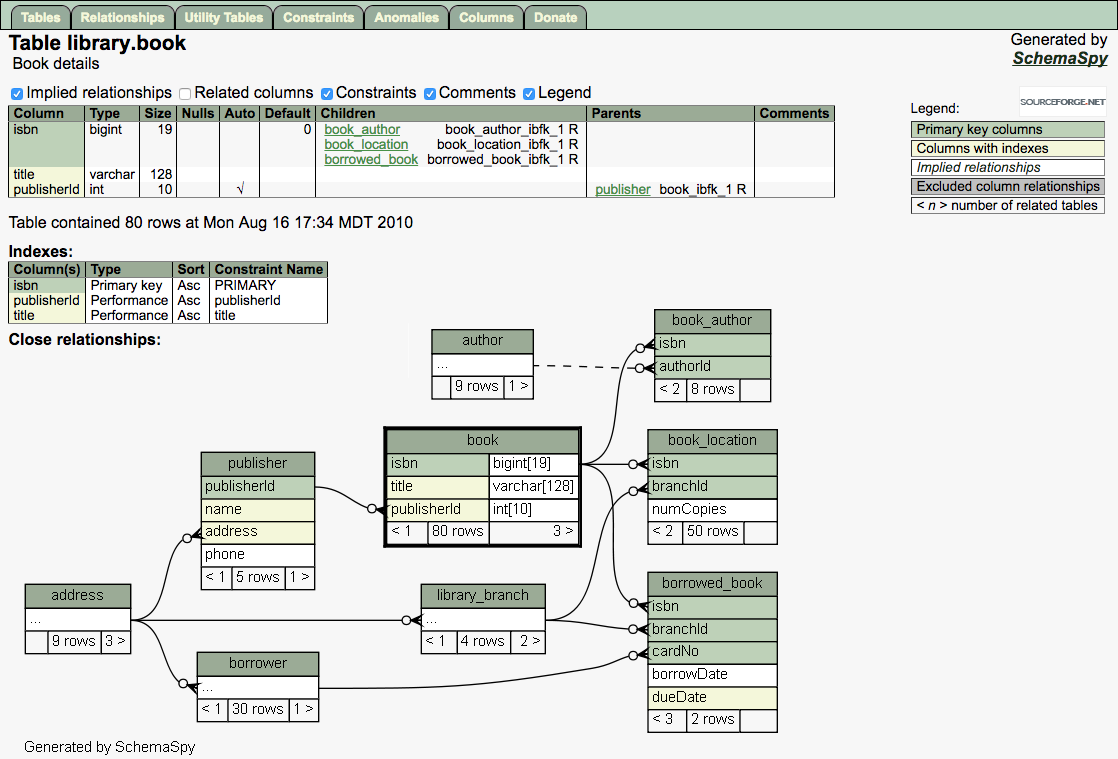
\includegraphics[width=0.85\textwidth]{bilder/datenbanken_SchemaSpy_Documentation}
  \end{center}
  \caption{Beispiel einer Dokumentation der Tabelle "`library.book"' mit Hilfe von SchemaSpy (http://schemaspy.sourceforge.net/sample/)}
  \label{abb:datenbanken-schemaspydoku}
\end{figure} 

Das Tool analysiert die Datenbank-Metadaten verschiedener DBMS, wie OracleDB, MySQL, PostgreSQL und MySQL, und erstellt unter anderem ein ERD aus der vorhandenen Datenstruktur, listet die Eigenschaften der Tabellen auf und visualisiert die Beziehungen zwischen ihnen. Es bietet damit eine wertvolle Unterstützung bei der Dokumentation der Datenstruktur, ersetzt jedoch nicht die inhaltliche und semantische Beschreibung von Tabellen, Attributen, Wertelisten und Sichten.

Ein weiteres Tool speziell für SQL"=Datenbanken ist der kostenlose ExPEditor, das eine Beschreibung der Datenbank im docx-Format generiert.

\begin{flushleft}
Schema Spy: \urllist{http://schemaspy.sourceforge.net/}
SchemaSpyGUI: \urllist{http://www.joachim-uhl.de/projekte/schemaspygui/}
ExPEditor: \urllist{http://www.yury-iwtschenko.de/de/expeditor.html}
\end{flushleft}

\subparagraph{Access-Datenbanken dokumentieren}
Microsoft Access bietet einige eingebaute Möglichkeiten, die die Erstellung einer Datenbank Dokumentation unterstützen. Ausführlicher werden die Möglichkeiten auf AccessDatabaseTutorial.com, bei Microsoft oder bei access-im-unternehmen.de erläutert.
\begin{itemize}
	\item Im Fenster Beziehungen (\emph{Microsoft Access 2010 $>$ Datenbanktools $>$ Beziehungen}) sind alle Tabellen der Access Datenbank inklusive ihrer Beziehungen untereinander dargestellt. Es ist auch möglich dieses Beziehungsdiagramm als Beziehungsbericht zu exportieren. (\emph{Microsoft Access 2010 $>$ Datenbanktools $>$ Beziehungen $>$ Entwurf $>$ Beziehungsbericht})
	\item Der Databanken Dokumentierer (\emph{Microsoft Access 2010 $>$ Datenbanktools $>$ Datenbankdokumentierer}) ermöglicht es automatisiert eine Dokumentation zu ausgewählten Objekten (Tabellen, Abfragen, Formularen, Berichten und Makros) zu erstellen. Das Textdokument kann nach Word exportiert werden.
	\item Das Database Preservation Toolkit unterstützt MS Access. Damit lässt sich die Datenbank mit Hilfe von SIARD archivieren. Mit SIARD kann auch die Datenbankstruktur beschrieben werden. Es wird jedoch empfohlen zusätzlich das Beziehungsdiagramm zu exportieren.
\end{itemize}

\begin{flushleft}
AccessDatabaseTutorial.com: \urllist{http://accessdatabasetutorial.com/2013/07/29/how-to-document-a-database-using-microsoft-access-tools-and-your-disciplines/}
Anleitung von Microsoft: \urllist{https://support.office.com/de-de/article/Dokumentieren-und-Drucken-des-Datenbankentwurfs-8bb56649-dd17-4d2e-b8dc-17dddd1ac91a}
Access im Unternehmen: \urllist{http://www.access-im-unternehmen.de/738}
\end{flushleft}

\subparagraph{Datenbanken mit SIARD archivieren}
Mit dem Format SIARD in der Version 2 lassen sich Datenbanken unabhängig von dem verwendeten DBMS sehr gut für die Archivierung vorbereiten. Die Erzeugung einer SIARD-Datei erfolgt mit dem Database Preservation Toolkit, das per Kommandozeile bedient wird. Die Software verbindet sich unter Angabe DBMS-spezifischer Parameter mit einer laufenden Datenbank, extrahiert die Struktur inklusive aller Attribute, Metadaten, Skripte sowie der Inhalte und transformiert alle Informationen in das SIARD-Format. Umgekehrt ermöglicht das Toolkit auch die Umwandlung einer SIARD-Datei in ein anderes DBMS-Format. Eine Beschreibung der Benutzung des Tools wird ebenfalls bereit gestellt.

\begin{flushleft}
Database Preservation Toolkit: \urllist{http://www.database-preservation.com/}
\end{flushleft}


\subparagraph{FileMaker-Datenbanken archivieren}
Das DBMS FileMaker Pro wird von den genannten Tools nicht unterstützt, da die Software anerkannte Standards, wie die Datenbanksprache SQL, nur eingeschränkt unterstützt. Daher muss bei der Archivierung und Dokumentation von FileMaker-Datenbanken ein individueller Ansatz gewählt werden, der hier skizziert wird.

Mit FileMaker Pro Advanced, einer erweiterten Version von FileMaker Pro, kann das Datenbankschema mit der Funktion "`Datenbank-Design-Report"' unter \emph{Werkzeuge $>$ Datenbank-Design-Report} in HTML oder XML dokumentiert werden. Die Funktion wird in der FileMaker Hilfe beschrieben.

Die Datenbankinhalte selbst lassen sich aus FileMaker Pro mit Hilfe von \emph{Datei $>$ Datensätze exportieren...} unter Windows, bzw. \emph{Ablage $>$ Datensätze exportieren...} unter MacOS im Format XML exportieren, wobei als XML-Grammatik \emph{FMPDSORESULT} verwendet werden sollte, um die Lesbarkeit zu erhalten.

\begin{figure}[!hbt]
	\lstset{language=XML}
	\begin{lstlisting}[frame=L, xleftmargin=0.3cm, rulecolor=\color{ianusGrau}, mathescape, basicstyle=\scriptsize]
	<?xml version="1.0" encoding="UTF-16"?>
	<FMPReport creationTime="14:38:43" creationDate="08.12.2016" 
						 type="Summary" version="11.0v3">
			<File link=".//Bleibarren_Bohrkern.xml" 
						name="Bleibarren_Bohrkern" path="134.95.117.58">
					<BaseTables count="3"/>
					<Tables count="37"/>
					<Relationships count="35"/>
					<Accounts count="4"/>
					<Privileges count="4"/>
					<ExtendedPrivileges count="6"/>
					<FileAccess count="0"/>
					<Layouts count="1"/>
					<Scripts count="10"/>
					<ValueLists count="87"/>
					<CustomFunctions count="1"/>
					<FileReferences count="13"/>
					<CustomMenuSets count="2"/>
					<CustomMenus count="30"/>
			</File>
	\end{lstlisting}
  \caption{Filemaker-Datenbank-Design-Bericht im XML-Format}
	\label{abb:datenbanken-berichtXML}
\end{figure}

\begin{flushleft}
Datenbank-Design-Report von Filemaker: \urllist{http://www.filemaker.com/de/help/html/fmpa_tools.24.5.html}
\end{flushleft}


%#############################################################

\paragraph{Quellen}
\begin{flushleft}
T. Bossert -- U. Böttcher -- P. Teich, SQL -- Grundlagen und Datenbankdesign (Bodenheim 2010).

H. Eiteljorg, Archaeological Computing $^2$(Bryn Mawr 2008) \urllist{http://archcomp.csanet.org/}

P. Kandzia -- H. J. Klein, Theoretische Grundlagen relationaler Datenbanksysteme. Reihe Informatik 79 (1993).

R. Elmasri -- S. B. Navathe. Fundamentals of Database Systems $^4$(2004).

A. Kemper -- A. Eickler, Datenbanksysteme. Eine Einführung $^7$(2009).

Koordinationsstelle für die dauerhafte Archivierung elektronischer Unterlagen (Hrsg.), Katalog archivischer Dateiformate: Datenbanken \urllist{http://kost-ceco.ch/wiki/whelp/KaD/pages/Datenbanken.html}

Library of Congress (Hrsg.), Sustainability of Digital Formats. Planning for Library of Congress Collections. Format Descriptions for Dataset Formats (12.2016) \urllist{http://www.digitalpreservation.gov/formats/fdd/dataset_fdd.shtml}

F. Schäfer -- K. Hofmann, Datenbankmanagementsysteme, in: DAI (Hrsg.), Leitfaden zur Anwendung von Informationstechniken der archäologischen Forschung. TEIL II Praxisratgeber (2011) \urllist{http://www.ianus-fdz.de/it-empfehlungen/sites/default/files/ianusFiles/IT-Leitfaden_Teil2_v100_DAI.pdf}

R. Steiner, Grundkurs relationale Datenbanken. Einführung in die Praxis für Ausbildung, Studium und IT-Beruf $^7$(Wiesbaden 2009).

P. Kleinschmidt -- Chr. Rank, Relationale Datenbanksysteme. Eine praktische Einführung $^3$(Berlin 2005).

G. Lock, Using Computers in Archaeology (London 2003) 85-98.

D. Smith, Database fundamentals for archaeologists, in: S. Ross et al. (Hrsg.), Computing for Archaeologists (Oxford 1991) 111-125.
	

\quelltyp{Formatspezifikationen}
SIARD 2.0: \urllist{http://www.ech.ch/vechweb/page?p=dossier&documentNumber=eCH-0165&documentVersion=2.0}
SIARD 1.0: \urllist{https://www.bar.admin.ch/dam/bar/de/dokumente/kundeninformation/siard_formatbeschreibung.pdf.download.pdf/siard_formatbeschreibung.pdf}
SQL:2008: ISO 9075 \urllist{http://www.iso.org/iso/catalogue_detail.htm?csnumber=45498 }
SQL:2011: ISO 9075 \urllist{http://www.iso.org/iso/iso_catalogue/catalogue_tc/catalogue_detail.htm?csnumber=53681}
Database Markup Language: \urllist{https://dml.codeplex.com/}
XML: W3C \urllist{http://www.w3.org/TR/xml/} 
CSV: RFC 4180 \urllist{https://tools.ietf.org/html/rfc4180}
JSON: \urllist{http://www.ecma-international.org/publications/standards/Ecma-404.htm}
ODB: \urllist{https://www.oasis-open.org/standards\#opendocumentv1.2}
ODB: \urllist{https://wiki.openoffice.org/wiki/FAQ_(Base)}

\quelltyp{Tools und Programme}
MySQL: \urllist{https://www.mysql.com/}
PostgreSQL: \urllist{https://www.postgresql.org/}
Vergleich von MySQL, PostgreSQL und SSLite: \urllist{https://www.digitalocean.com/community/tutorials/sqlite-vs-mysql-vs-postgresql-a-comparison-of-relational-database-management-systems}
Microsoft SQL Server: \urllist{https://www.microsoft.com/en-us/sql-server/sql-server-2016}
Oracle: \urllist{https://www.oracle.com/database/index.html}
FileMaker Pro: \urllist{http://www.filemaker.com/}
Microsoft Access: \urllist{https://products.office.com/de-DE/access}
OpenOffice Base: \urllist{https://www.openoffice.org/product/base.html}
SQLite: \urllist{https://sqlite.org/}
pgAdmin3: \urllist{https://www.pgadmin.org/}
MySQL Workbench: \urllist{http://www.mysql.de/products/workbench/}
SQLite Database Browser: \urllist{http://sqlitebrowser.org/}
Oracle SQL Developer: \urllist{http://www.oracle.com/technetwork/developer-tools/sql-developer/}
SQL Server Management Studio: \urllist{https://msdn.microsoft.com/de-de/library/mt238290.aspx}
SQuirrel SQL: \urllist{http://squirrel-sql.sourceforge.net/}
phpmyadmin: \urllist{https://www.phpmyadmin.net/}
phppgadmin: \urllist{http://phppgadmin.sourceforge.net/}
Adminer: \urllist{https://www.adminer.org/}
Schema Spy: \urllist{http://schemaspy.sourceforge.net/}
SchemaSpyGUI: \urllist{http://www.joachim-uhl.de/projekte/schemaspygui/}
Database Preservation Toolkit: \urllist{http://www.database-preservation.com/}
Nutzung des Tools: \urllist{http://www.database-preservation.com/}
Datenbank-Design-Report von Filemaker: \urllist{http://www.filemaker.com/de/help/html/fmpa_tools.24.5.html}
\end{flushleft}